\documentclass[ngerman,a4paper,order=firstname]{../../texmf/tex/latex/mathscript/mathscript}
\usepackage{../../texmf/tex/latex/mathoperators/mathoperators}

\title{\textbf{Geometrie WS2018/19}}
\author{Dozent: Prof. Dr. \person{Arno Fehm}}

\begin{document}
\pagenumbering{roman}
\pagestyle{plain}

\maketitle

\hypertarget{tocpage}{}
\tableofcontents
\bookmark[dest=tocpage,level=1]{Inhaltsverzeichnis}

\pagebreak
\pagenumbering{arabic}
\pagestyle{fancy}

\chapter*{Vorwort}
Schön, dass du unser Skript für die Vorlesung \textit{Lineare Algebra und analytische Geometrie 1} bei Prof. Dr. Arno Fehm im WS2017/18 gefunden hast! \footnote{Obwohl man sagen kann, dass es in dieser Vorlesung nur um Lineare Algebra ging, der Teil mit der analytischen Geometrie wurde vernachlässigt. Liegt wahrscheinlich auch daran, dass es demnächst eine Reform der Studienordnung gibt, in der aus der Vorlesung \textit{Lineare Algebra und analytische Geometrie} die Vorlesung \textit{Einführung in die Lineare Algebra} wird.}

Wir verwalten dieses Skript mittels Github \footnote{Github ist eine Seite, mit der man Quelltext online verwalten kann. Dies ist dahingehend ganz nützlich, dass man die Quelltext-Dateien relativ einfach miteinander synchronisieren kann, wenn man mit mehren Leuten an einem Projekt arbeitet.}, d.h. du findest den gesamten \LaTeX-Quelltext auf \url{https://github.com/henrydatei/TUD_MATH_BA}. Unser Ziel ist, für alle Pflichtveranstaltungen von \textit{Mathematik-Bachelor} ein gut lesbares Skript anzubieten. Für die Programme, die in den Übungen zur Vorlesung \textit{Programmieren für Mathematiker} geschrieben werden sollen, habe ich ein eigenes Repository eingerichtet; es findet sich bei \url{https://github.com/henrydatei/TU_PROG}.

Du kannst dir gerne dort die \LaTeX-Quelldateien herunterladen, die Dateien für exakt dieses Skript sind im Ordner \texttt{1. Semester/LAAG ueberarbeitet}. Es lohnt sich auf jeden Fall während des Studiums die Skriptsprache \LaTeX{} zu lernen, denn Dokumente, die viele mathematische oder physikalische Formeln enthalten, lassen sich sehr gut mittels \LaTeX{} darstellen, in Word oder anderen Office-Programmen sieht so etwas dann eher dürftig aus.

\LaTeX{} zu lernen ist gar nicht so schwierig, ich habe dafür am Anfang des ersten Semesters wenige Wochen benötigt, dann kannte ich die wichtigsten Befehle und konnte den Vorgänger dieses Skriptes schreiben (\texttt{1. Semester/LAAG}, Vorsicht: hässlich, aber der Quelltext ist relativ gut verständlich).

Es sei an dieser Stelle darauf hingewiesen (wie in jedem anderem Skript auch \smiley{}), dass dieses Skript nicht den Besuch der Vorlesungen ersetzen kann. Es könnte sein, dass Prof. Fehm seine Vorlesung immer mal wieder an die Studenten anpasst; wahrscheinlich immer dann, wenn die Prüfungsergebnisse zu schlecht waren. Nichtsdestotrotz veröffentlicht Prof. Fehm sein Skript auf seiner Homepage \url{http://www.math.tu-dresden.de/~afehm/lehre.html}. Allerdings ist dieses Skript recht hässlich, besonders was die Übersichtlichkeit angeht.

Wir möchten deswegen ein Skript bereitstellen, dass zum einen übersichtlich ist, zum anderen \textit{alle} Inhalt aus der Vorlesung enthält, das sind insbesondere Diagramme, die sich nicht im offiziellen Skript befinden, aber das Verständnis des Inhalts deutlich erleichtern. Ich denke, dass uns dies erfolgreich gelungen ist.

Trotz intensivem Korrekturlesen können sich immer noch Fehler in diesem Skript befinden. Es wäre deswegen ganz toll von dir, wenn du auf unserer Github-Seite \url{https://github.com/henrydatei/TUD_MATH_BA} ein neues Issue erstellst und damit auch anderen hilfst, dass dieses Skript immer besser wird.

\chapter{Endliche Gruppen}
\section{Erinnerung und Beispiele}

\begin{erinnerung}
	Ein \begriff{Ring} ist eine abelsche Gruppe $(R,+)$ zusammen mit einer Verknüpfung $\cdot : R\times R \to R$ die Assoziativität und Distributivität erfüllt. Eine Teilmenge $\emptyset \neq S \subseteq R$ ist ein \begriff{Unterring} oder \begriff{Teilring} von $R$, wenn $S$ abgeschlossen unter Addition, Subtraktion und Multiplikation ist. Eine Abbildung $\phi : R \to R^{'}$ zwischen Ringen ist ein \begriff{Ringhomomorphismus}, wenn $\phi(r_1 + r_2) = \phi(r_1) + \phi(r_2) \text{ und } \phi(r_1 r_2) = \phi(r_1) \phi(r_2)$ und in diesem Fall ist
	\begin{align}
		\ker(\phi)=\phi^{-1}(\{0\}) \notag
	\end{align}
	der \begriff{Kern} von $\phi$.
\end{erinnerung}

\begin{remark}
	In dieser Vorlesung bedeutet ``Ring'' \emph{immer} kommutativer Ring mit Einselement, d.h. $(R,\cdot)$ bildet ein kommutativer Monoid mit Einselement $1_R$. Wir fordern dann zusätzlich, dass Unterringe von $R$ das Einselement von $R$ enthalten und dass Ringhomomorphismen $\phi : R \to R^{'}$ das Einselement von $R$ auf das Einselement von $R^{'}$ abbilden.
\end{remark}

\begin{example}
	\begin{enumerate}
		\item Der Ring $\whole$ der ganzen Zahlen.
		\item Der Restklassenring $\whole / n \whole$ für $n \in \natur$.
		\item Die Körper $\ratio, \real, \comp$.
		\item Der Nullring $R = \{0\}$
	\end{enumerate}
\end{example}

Seien $R, S$ Ringe. (Meisten Beweise sind LAAG1+2 Skript zu entnehmen!)

\begin{proposition}
	Ein Ringhomomorphismus $\phi: R \to S$ ist ein Isomorphismus (d.h. bijektiv), wenn es einen Ringhomomorphismus $\psi: S \to R$ mit $\psi \circ \phi = \id_R$ und $\phi \circ \psi = \id_{S}$ gibt.
\end{proposition}

\begin{proposition}
	Ein Ringhomomorphismus $\phi: R \to S$ ist genau dann injectiv, wenn $\ker(\phi) =\{0\}$.
\end{proposition}

\begin{definition}
	Für $x \in R$ heißt \begriff{invertierbar} oder eine \begriff{Einheit}, wenn es $y\in R$ mit $xy=1$ gibt, und die $R^{\times}$ der Einheiten bildet eine Gruppe unter Multiplikation.\\
	Für $x \in R$ ist eine \begriff{Nullteiler}, wenn es $0 \neq y \in R$ mit $xy=0$ gibt, und $R$ ist \begriff{nullteilerfrei}, wenn es keinen Nullteiler $0\neq x \in R$ gibt.
\end{definition}

\begin{example}
	\begin{enumerate}
		\item $\whole$ ist nullteilerfrei, $\whole^{\times} = \mu_2 = \{ \pm 1 \}$.
		\item $\whole / n \whole$ ist genau dann nullteilerfrei, wenn $n$ prim ist.
	\end{enumerate}
\end{example}

\begin{example}
	Für eine Familie von Ringen $(R_i)_{i \in I}$ wird $\prod_{i \in \Lambda} R_i$ durch komponentenweise Addition und Multiplikation zu einem Ring, genannt das \begriff{direkte Produkt} der $R_i$. Bezeichnet $1_{R_i}$ das Einselement von $R_i$, so ist $(1_{R_i})$ das Einselement von $\prod_{i \in \Lambda} R_i$ und 
	\begin{align}
		\left(\prod_{i\in \Lambda} R_i\right)^{\times} = \prod_{i \in I}R_i \notag
	\end{align}
\end{example}

\begin{example}
	Der \begriff{Polynomring} eine Variablen $x$ über $R$ ist 
	\begin{align}
		R[x] = \left\{ \sum_{i=0}^{\infty} a_i x^i \mid a_i \in R, \text{ fast alle } a_i = 0\right\} \notag
	\end{align}
	mit der Addition und Multiplikation
	\begin{align}
		\sum_{i=0}^{\infty} a_i x^i + \sum_{i=0}^{\infty} b_i x^i &= \sum_{i=0}^{\infty} (a_i + b_i) x^i \notag \\
		\left(\sum_{i=0}^{\infty} a_i x^i\right) + \left(\sum_{j=0}^{\infty} b_j x^j\right) &= \sum_{k=0}^{\infty} \left(\sum_{i+j=k}^{\infty} a_i b_j\right) x^k \notag
	\end{align}
	Ist $f = \sum_{i=0}^n a_i x^i \in R[x]$ mit $a_n \neq 0$, so ist $\deg(f) = n$ der \begriff{Grad} von $f$ (mit $\deg(0) = -\infty$) und $\LC(f) = a_n$ der \begriff{Leitkoeffizient} von $f$, $f$ heißt \begriff{normiert}, wenn $\LC(f) = 1$.
\end{example}

\begin{proposition}
	\proplbl{2_1_10}
	Seien $f,g \in R[x]$.
	\begin{enumerate}
		\item $\deg(f + g) \leq \max\{ \deg(f), \deg(g) \}$
		\item $\deg(f \cdot g) \leq \deg(f) + \deg(g)$
		\item Ist $f \neq 0$ und $\LC(f)$ kein Nullteiler, so ist $\deg(fg) = \deg(f) + \deg(g)$.
	\end{enumerate}
\end{proposition}

\begin{proof}
	Siehe LAAG I.6.4.
\end{proof}

\begin{conclusion}
	Ist $R$ nullteilerfrei, so auch $R[x]$ und $(R[x])^{\times} = R^{\times}$.
\end{conclusion}

\begin{proof}
	\begin{itemize}
		\item Ist $fg=0$, so ist
		\begin{align}
		-\infty = \deg(0) = \deg(fg) \overset{\propref{2_1_10}}{=} \deg(f) + \deg(g) \notag
		\end{align}
		folglich $f=0$ oder $g=0$.
		\item 	Ist $fg = 1$, so ist
		\begin{align}
		0 = \deg(1) = \deg(fg) \overset{\propref{2_1_10}}{=} \deg(f) + \deg(g) \notag
		\end{align}
		folglich $\deg(f) = \deg(g) = 0$, d.h. $f,g \in R$.
	\end{itemize}
\end{proof}

\begin{proposition}[Universelle Eigenschaft des Polynomrings]
	\proplbl{2_1_12}
	Ist $\phi : R \to S$ ein Ringhomomorphismus und $s \in S$, so gibt es genau einen Ringhomomorphismus $\phi_s : R[x] \to S$ mit 
	\begin{align}
	\phi_{s}|_R = \phi \text{ und } \phi_{s} (x) = S\notag
	\end{align}
\end{proposition}

\begin{proof}
	Ist $R[x] \to S$ ein Ringhomomorphismus mit $\phi_{s}|_R = \phi$ und $\phi_{s(x)} = S$, so ist
	\begin{align}
		\phi_{s}\left(\sum_{i\geq 0}^{\infty} a_i x^i\right) = \sum_{i=0}^{\infty} \phi_{s}(a_i) \phi_{s}(x^i) = \sum_{i\geq 0}^{\infty} \phi(a_i) s^i \notag
	\end{align}
		eindeutig bestimmt. Umgekehrt ist das so definierte $\phi_s$ ein Ringhomomorphismus (Übung), der $\phi_{s}|_R$ und $\phi_{s}(x) = s$ erfüllt.
\end{proof}

\begin{remark}
	Insbesondere hat man für $a\in R$ den Einsetzungshomomorphismus:
	\begin{align}
		\varphi_{a}: \begin{cases}
		R[x] &\to R \\
		f &\mapsto f(a) 
		\end{cases}\notag
	\end{align}
	gegeben durch $\varphi_{a}\mid_{R} = \id_R$ und $\varphi_{a}(x) = a$. Dies liefert eine Abbildung
	\begin{align}
	\begin{cases}
	R[x] &\to \Abb(R,R) \\
	f &\mapsto \tilde{f}, \tilde{f}(a) = \varphi_a(f) 
	\end{cases}\notag
	\end{align}
	Diese Abbildung ist im Allgemeinen \emph{nicht injectiv}!!! Sei z.B. für $R = \whole / n\whole$ und $f = x^2 + x$ ist $f(0) = \overline{0}$, $f(\overline{1}) = \overline{0}$, aber $\tilde{f} = \tilde{0}$, aber $f\neq 0$.
\end{remark}

\begin{proposition}[Polynomdivision]
	\proplbl{2_1_14}
	Sei $0 \neq g \in R[x]$ mit $\LC(g) \in R^{\times}$. Zu jedem Polynom $f \in R[x]$ gibt es eindeutig bestimmte $q_{1}r \in R[x]$ mit $f = qg +r$ und $\deg(r) < \deg(g)$.
\end{proposition}

\begin{proof}
	Wie im Falle $R = K$ ein Körper.
	\begin{itemize}
		\item \textbf{Eindeutigkeit:} Sei $f = q_1 g+ r_1 = q_2 g + r_2$ und $\deg(r_1) <\deg(g) \Rightarrow r_1 - r_2 = (q_2 - q_1)g$. Da $\LC(g) \in R^{\times}$ ist $\LC(g)$ kein Nullteiler $\overset{\propref{2_1_10}}{\Rightarrow} \deg(r_1 - r_2) < \deg(g) = \deg(q_2 - q_1) + \deg(g)$ \\
		$\Rightarrow \deg(q_2 - q_1) < 0 \Rightarrow q_1 = q_2$ und $r_1 = r_2$
		\item \textbf{Existenz:} Sei $f = \sum_{i=0}^{n} a_i x^i$, $a_n \neq 0$ und $g = \sum_{j=0}^{m} b_j x^j$ mit $b_m \neq 0$. Nach Vorraussetzung ist $b_m \in R^{\times}$ es existiert also $b_m^{-1} \in R$.\\
		Induktion nach $\deg(f) = n$:
		\begin{itemize}
			\item \textbf{$n < m$:} $q = 0$, $r = f$
			\item \textbf{$n\geq m$:} $f_i = f - a_n b_m^{-1} x^{n-m} \cdot g \Rightarrow \deg(f_1) < \deg(f)$ mit Induktionshypothese folgt $f_1 = q_1 \cdot g + r_1$ mit $\deg(r) < m$ $\Rightarrow f = (q_1 + a_n b_m^{-1} x^{n-m})g + r$
		\end{itemize}
	\end{itemize}
\end{proof}

\begin{conclusion}
	Ist $f \in R[x]$ und $a \in R$, $f(a) = 0$, so ist
	\begin{align}
		f(x) = (x-a)\cdot q(x) \text{ mit } q \in R[x]. \notag
	\end{align}
\end{conclusion}

\begin{proof}
	Sei $f = q(x-a) + r$, $\deg(r) < \deg(x-a)$, d.h. $\deg(1) \leq 0 \Rightarrow 0 = f(a) = q(a-a) + r(a) \Rightarrow r(a) = 0$.
\end{proof}

\begin{conclusion}
	\proplbl{2_1_16}
	Ist $R$ nullteilerfrei, so hat $0 = f \in R[x]$ höchstens $\deg(f)$ viele Nullstellen in $R$.
\end{conclusion}

\begin{definition}[Polynomring in kommutieren Variablen]
	Für eine Menge $I$ definieren wir den Monoid
	\begin{align}
	\natur_{0}^{(I)} : = \left\{ (\mu_i)_{i \in I} \in \prod_{i \in I} \natur_{0} \colon \mu_i = 0 \text{ für fast alle } i \right\}\notag
	\end{align}
	mit Addition
	\begin{align}
		(\mu_i)_{i \in I} + (\nu_i)_{i \in I} :=(\mu_i+\nu_i)_{i \in I}, \notag
	\end{align}
	sowie den Ring
	\begin{align}
		R[x_i \colon i \in I] = \{ (_{\mu})_{\mu \in \natur_{0}} \colon a_{\mu} \in R, \text{ fast alle gleich } 0\} \notag
	\end{align}
	mit Addition und Multiplikation
	\begin{align}
		(a_{\mu})_{\mu \in \natur_{0}}^{(I)} + (b_{\mu})_{\mu \in \natur_{0}}^{(I)} &:= (a_{\mu} + b_{\mu})_{\mu \in \natur_{0}}^{(I)}\notag \\
		(a_{\lambda})_{\lambda \in \natur_{0}^{(I)}}\cdot (b_{\nu})_{\nu \in \natur_{0}^{(I)}} &:= \left( \sum_{\lambda + \nu = \mu} a_{\lambda}b_{\mu}\right)_{\mu \in \natur_{0}}^{(I)}, \notag
	\end{align}
	gennant \begriff{Polynomring in kommutierenden Variablen} $x_i, i \in I$. Wir identifizieren den Ring $R$ mit den Unterring
	\begin{align}
		\{ (r\delta_{\mu,\underline{0}})_{\mu \in \natur_{0}}^{(I)}\colon r \in R \}. \notag
	\end{align}
	Wir schreiben $x_i := (\delta_{\mu\nu})_{\mu \in \natur_{0}}^{(I)}$, $\mu := (\delta_{ij})_{i \in I}$ und $x^{\mu} := \prod_{i \in I}x_i^{\mu_i}$. Damit ist dann
	\begin{align}
		(a_{\mu})_{\mu \in \natur_{0}}^{(I)} = \sum_{\mu \in \natur_{0}^{(I)}} a_{\mu} x^{\mu}. \notag
	\end{align}
	Weiter schreiben wir
	\begin{align}
		R[x_1, \dots, x_n] := R[x_i \colon i \in \{ i, \dots, n \}]. \notag
	\end{align}
\end{definition}

\begin{example}
	Sei $R = \whole$ und $I = \{1,2\}$, dann
	\begin{align}
		\left( x_1 x_2 + x_2^2 \right)^2 = a_{(2,1)}x_1^2 x_2^2 + a_{(1,3)}x_1 x_2^2 + a_{(0,4)}x_2^4\notag	
	\end{align}
	mit $a_{(2,1)} = 1$, $a_{(1,3)} = 2$ und $a_{(0,4)} = 1$
\end{example}

\begin{remark}
	\propref{2_1_10} und \propref{2_1_12} kann man allgemein für $R[x_i \colon i \in I]$ anstatt $R[x]$ formulieren. Für \propref{2_1_14} - \propref{2_1_16} gibt es keine Verallgeminerung. So hat z.B. $f = x_1 - x_2$ unendlich viele Nullstellen, da $f(a,a) = 0$ für alle $a \in \whole$.
\end{remark}
\section{Ordnung und Index}

Sei $G$ eine Gruppe, $g\in G$.

\begin{definition}[Ordnung]
	\begin{enumerate}[label=(\alph*)]
		\item $\#G=\vert G\vert\in\natur\cup\{\infty\}$, die \begriff{Ordnung} von $G$.
		\item $\ord(g)=\#\langle g\rangle$, die \underline{Ordnung} von $g$.
	\end{enumerate}
\end{definition}

\begin{example}
	\begin{enumerate}[label=(\alph*)]
		\item $\# S_n=n!$
		\item $\# A_n=\frac{1}{2}n!$ für $n\ge 2$
		\item $\#\whole/n\whole=n$
	\end{enumerate}
\end{example}

\begin{lemma}
	\proplbl{1_2_3}
	Für $X\subseteq G$ ist
	\begin{align}
		\langle X\rangle = \{g_1^{\varepsilon_1}\cdot\dots\cdot g_r^{\varepsilon_r}\mid r\in\natur_0,g_1,...,g_r\in X, \varepsilon_1,...,\varepsilon_r\in\{-1,1\}\}\notag
	\end{align}
\end{lemma}
\begin{proof}
	klar, rechte Seite ist Untergruppe, die $X$ enthält, und jede solche enthält alle Ausdrücke der Form  $g_1^{\varepsilon_1}\cdot\dots\cdot g_r^{\varepsilon_r}$.
\end{proof}

\begin{proposition}
	\proplbl{1_2_4}
	\begin{enumerate}[label=(\alph*)]
		\item Ist $\ord(g)=\infty$, so ist $\langle g\rangle=\{...,g^{-2},g^{-1},1,g^1,g^2,...\}$
		\item Ist $\ord(g)=n$, so ist $\langle g\rangle=\{1,g,g^2,...,g^{n-1}\}$
		\item Es ist $\ord(g)=\inf\{k\in\natur\mid g^k=1\}$
	\end{enumerate}
\end{proposition}
\begin{proof}
	Nach \propref{1_2_3} ist $\langle g\rangle=\{g^k\mid k\in\whole\}$. Sei $m=\inf\{k\in\natur\mid g^k=1\}$.
	\begin{itemize}
		\item $\vert\{k\in\natur\mid g^k=1\}\vert=m$: Sind $g^a=g^b$ mit $0\le a<b<m$, so ist $g^{b-a}=1$, aber $0<b-a<m$, was ein Widerspruch zur Minimalität von $m$ ist.
		\item $m=\infty\Rightarrow\ord(g)=\infty$: klar
		\item $m<\infty\Rightarrow\langle g\rangle=\{g^k\mid 0\le k<m\}$: Für $k\in\whole$ schreibe $k=qm+r$ mit $q,r\in\whole$ und $0\le r<m$
		\begin{align}
			g^k=g^{qm+r}=(\underbrace{g^m}_{=1})^q\cdot g^r=g^r\in{^1,g,...,g^{m-1}}\notag
		\end{align}
	\end{itemize}
\end{proof}

\begin{example}
	\begin{enumerate}[label=(\alph*)]
		\item Ist $\sigma\in S_n$ ein $k$-Zykel, so ist $\ord(\sigma)=k$.
		\item Für $\overline{1}\in\whole/n\whole$ ist $\ord(\overline{1})=n$.
	\end{enumerate}
\end{example}

\begin{definition}[Komplexprodukt, Nebenklasse]
	Seien $A,B\subseteq G$, $H\le G$
	\begin{enumerate}[label=(\alph*)]
		\item $AB:=A\cdot B:=\{ab\mid a\in A,b\in B\}$ das \begriff{Komplexprodukt} von $A$ und $B$.
		\item $gH:=\{g\}\cdot H=\{gh\mid h\in H\}$ die \begriff{Linksnebenklasse} von $H$ bezüglich $g$. \\
		$Hg:=H\cdot \{g\}=\{hg\mid h\in H\}$ die \begriff{Rechtsnebenklasse} von $H$ bezüglich $g$.
		\item $\lnkset{G}{H}:=\{gH\mid g\in G\}$ die Menge der Linksnebenklassen. \\
		$\rnkset{G}{H}:=\{Hg\mid g\in G\}$ die Menge der Rechtsnebenklassen.
	\end{enumerate}
\end{definition}

\begin{example}
	Für $h\in H$ ist $hH=H=Hh$.
\end{example}

\begin{lemma}
	\proplbl{1_2_8}
	Seien $H\le G$, $g,g'\in G$.
	\begin{enumerate}[label=(\alph*)]
		\item $gH=g'H\Leftrightarrow g'=gh$ für ein $h\in H$ \\
		$Hg=Hg'\Leftrightarrow g'=gh$ für ein $h\in H$
		\item Es ist $gH=g'H$ oder $gH\cap g'H=\emptyset$ und $Hg=Hg'$ oder $Hg\cap Hg'=\emptyset$.
		\item Durch $gH\mapsto Hg^{-1}$ wird eine wohldefinierte Bijektion $\lnkset{G}{H}\to\rnkset{G}{H}$ gegeben.
	\end{enumerate}
\end{lemma}
\begin{proof}
	\begin{enumerate}[label=(\alph*)]
		\item Hinrichtung: $gH=g'H\Rightarrow g'=g'\cdot 1\in g'H=gH\Rightarrow$ es existiert $h\in H$ mit $g'=gh$ \\
		Rückrichtung: $g'=gh\Rightarrow g'H=ghH=gH$
		\item Ist $gH\cap g'H\neq\emptyset$, so existieren $h,h'\in H$ mit $gh=g'h'\Rightarrow gH=ghH=g'h'H=g'H$
		\item wohldefiniert: $gH=g'H\overset{a)}{\Rightarrow}g'=gh$ mit $h\in H\Rightarrow H(g')^{-1}=Hh^{-1}g^{-1}=Hg^{-1}$ \\
		bijektiv: klar, Umkehrabbildung: $Hg\mapsto g^{-1}H$ 
	\end{enumerate}
\end{proof}

\begin{definition}[Index]
	Für $H\subseteq G$ ist
	\begin{align}
		(G:H):=\vert\lnkset{G}{H}\vert + \vert\rnkset{G}{H}\vert\in\natur\cup\{\infty\}\notag
	\end{align}
	der \begriff{Index} von $H$ in $G$.
\end{definition}

\begin{example}
	\begin{enumerate}[label=(\alph*)]
		\item $(S_n:A_n)=2$ für $n\ge 2$
		\item $(\whole:n\whole)=n$
	\end{enumerate}
\end{example}

\begin{proposition}
	\proplbl{1_2_11}
	Der Index ist multiplikativ: Sind $K\le H\le G$, so ist
	\begin{align}
		(G:K)=(G:H)\cdot (H:K)\notag
	\end{align}
\end{proposition}
\begin{proof}
	Nach \propref{1_2_8} bilden die Nebenklassen von $H$ eine Partition von $G$, das heißt es gibt $(g_i)_{i\in I}$ in $G$ mit $G=\biguplus_{i\in I}g_iH$. Analog ist $H=\biguplus_{j\in J}h_jK$ mit $h_j\in H$. Dann gilt:
	\begin{align}
		H &= \biguplus_{j\in J} h_jK\overset{\propref{1_1_4}}{\Rightarrow} gH=\biguplus_{j\in J} gh_jK\text{ für jedes }g\in G \notag\\
		G &= \biguplus_{i\in I} g_iH=\biguplus_{i\in I}\biguplus_{j\in J} g_ih_jK=\biguplus_{(i,j)\in I\times J} g_ih_jK \notag
	\end{align}
	Somit ist $(G:K)=\vert I\times J\vert=\vert I\vert\cdot\vert J\vert=(G:H)\cdot (H:K)$.
\end{proof}

\begin{conclusion}[Satz von \person{Lagrange}]
	\proplbl{1_2_12}
	Ist $G$ endlich und $H\le G$, so ist
	\begin{align}
		\# G=\#H\cdot (G:H)\notag
	\end{align}
	Insbesondere gilt $\#H\vert\# G$ und $(G:H)\vert \#G$.
\end{conclusion}
\begin{proof}
	$\# G=(G:1)\overset{\propref{1_2_11}}{=}(G:H)(H:1)=(G:H)\cdot\#H$.
\end{proof}

\begin{conclusion}[kleiner Satz von \person{Fermat}]
	Ist $G$ endlich und $n=\# G$, so ist $g^n=1$ für jedes $g\in G$.
\end{conclusion}
\begin{proof}
	Nach \propref{1_2_12} gilt: $\ord(g)=\#\langle g\rangle\vert \#G=n$. Nach \propref{1_2_4} ist $g^{\ord(g)}=1$, somit auch
	\begin{align}
		g^n=(\underbrace{g^{\ord(g)}}_{=1})^{\frac{n}{\ord(g)}}=1\notag
	\end{align}
\end{proof}

\begin{remark}
	Nach \propref{1_2_12} ist die Ordnung jeder Untergruppe von $G$ ein Teiler der Gruppenordnung $\# G$. Umgekehrt gibt es im Allgemeinen aber nicht zu jedem Teiler $d$ von $\# G$ eine Untergruppe $H$ von $G$ mit $\# H=d$.
\end{remark}
\section{Normalteiler und Quotientengruppen}

Sei $G$ eine Gruppe.

\begin{definition}[normal, Normalteiler]
	Eine Untergruppe $H\le G$ ist \begriff{normal} (in Zeichen $H\unlhd G$), wenn $g^{-1}hg\in H$ für alle $h\in H$ und $g\in G$. Ein \begriff{Normalteiler} von $G$ ist eine normale Untergruppe von $G$.
\end{definition}

\begin{example}
	\begin{enumerate}[label=(\alph*)]
		\item Ist $G$ abelsch, so ist jede Untergruppe von $G$ ein Normalteiler.
		\item Ist $\phi: G\to H$ ein Gruppenhomomorphismus, so ist $\Ker(\phi)\unlhd G$, denn $\phi(h)=1\Rightarrow\phi(g^{-1}hg)=\phi(g)^{-1}\phi(h)\phi(g)=1$ $\forall g\in G$.
		\item Jede Gruppe $G$ hat die trivialen Normalteiler $1\unlhd G$ und $G\unlhd G$.
	\end{enumerate}
\end{example}

\begin{lemma}
	\proplbl{1_3_3}
	Sei $H\le G$ und $N\unlhd G$.
	\begin{enumerate}[label=(\alph*)]
		\item $H\unlhd G\Leftrightarrow gH=Hg$ für alle $g\in G$
		\item $HN=NH$, $HN\le G$, $N\unlhd HN$, $H\cap N\le N$, $H\cap N\unlhd H$
		\item Sind $N,H\unlhd G$, so ist $H\cap N\unlhd G$, $HN\unlhd G$
		\item Für $g,g'\in G$ ist $gN\cdot g'N=gg'N$
	\end{enumerate}
\end{lemma}
\begin{proof}
	\begin{enumerate}[label=(\alph*)]
		\item Hinrichtung: $\forall g\in G$, $\forall h\in H$: $g^{-1}hg\in H\Rightarrow gHg^{-1}\subseteq H\Rightarrow Hg=gH$ und $g^{-1}H\subseteq Hg^{-1}\Rightarrow gH=Hg$ \\
		Rückrichtung: $\forall g\in G$: $gH=Hg \Rightarrow\exists h'\in H$: $gh'=hg\Rightarrow g^{-1}hg=h\in H$
		\item \begin{itemize}
			\item $HN=\bigcup_{n\in\natur} hN=\bigcup_{n\in\natur} Nh=NH$
			\item $HN\cdot NH=H\cdot NH\cdot N=H\cdot HN\cdot N=HN$ \\
			$(HN)^{-1}=N^{-1}H^{-1}=NH=HN$
			\item $N\unlhd HN$: klar
			\item $H\cap N\le N$: klar
			\item $H\cap N\unlhd H$: $n\in H\cap N$, $h\in H\Rightarrow h^{-1}nh\in H\cap N$
		\end{itemize}
		\item \begin{itemize}
			\item $H\cap N\unlhd G$: $h\in H\cap N$, $g\in G\Rightarrow g^{-1}hg\in H\cap N$
			\item $HN\unlhd G$: $g\in G\Rightarrow gHN\overset{a)}{=}Hg\cdot N=H\cdot gN\overset{a)}{=}H\cdot Ng=HNg$
		\end{itemize}
		\item $gN\cdot g'N=g\cdot Ng'\cdot N\overset{a)}{=}g\cdot g'N=gg'N$
	\end{enumerate}
\end{proof}

\begin{proposition}
	Sei $N\unlhd G$. Dann ist $\lnkset{G}{N}$ mit dem Komplexprodukt als Verknüpfung eine Gruppe, und $\pi_N:G\to\lnkset{G}{N}$, $g\mapsto gN$ ein Gruppenhomomorphismus mit Kern $N$.
\end{proposition}
\begin{proof}
	\begin{itemize}
		\item Komplexprodukt ist Verknüpfung auf $\lnkset{G}{N}$: \propref{1_3_3}
		\item Gruppenaxoime übertragen sich von $G$ auf $\lnkset{G}{N}$: klar
		\item $\pi_N$ ist ein Homomorphismus: \propref{1_3_3}
		\item $\Ker(\pi_N)=N$: \propref{1_2_8}
	\end{itemize}
\end{proof}

\begin{conclusion}
	Die Normalteiler sind genau die Gruppenhomomorphismen.
\end{conclusion}

\begin{definition}[Quotientengruppe]
	Für $N\unlhd G$ heißt $\lnkset{G}{N}$ zusammen mit dem Komplexprodukt als Verknüpfung die \begriff{Quotientengruppe} von $G$ nach $N$ (oder $G$ modulo $N$).
\end{definition}

\begin{lemma}
	\proplbl{1_3_7}
	Sei $N\unlhd G$. Für $H\le G$ ist $\pi_N(H)=\lnkset{HN}{N}\le\lnkset{G}{N}$, und $H\mapsto \pi(H)$ liefert eine Bijektion zwischen 
	\begin{itemize}
		\item den $H\le G$ mit $N\le H$ und
		\item den $H\le\lnkset{G}{N}$
	\end{itemize}
\end{lemma}
\begin{proof}
	\begin{itemize}
		\item $\pi_N(H)=\{hN\mid h\in H\}=\{hnN\mid h\in H, n\in N\}=\lnkset{HN}{N}$
		\item Umkehrabbildung: $H\mapsto \pi_N^{-1}(H)$: \\
		$H\le\lnkset{G}{N}$: $\pi_N(\pi_N^{-1}(H))=H$, da $\pi_N$ surjektiv \\
		$N\le H\le G$: $\pi_N^{-1}(\pi_N(H))=\pi_N^{-1}(\lnkset{HN}{N})=HN\subseteq H\cdot H=H$
	\end{itemize}
\end{proof}

\begin{proposition}[Homomorphiesatz]
	\proplbl{1_3_8}
	Sei $\phi:G\to H$ ein Gruppenhomomorphismus und $N\unlhd G$ mit $N\le \Ker(\phi)$. Dann gibt es genau einen Gruppenhomomorphismus $\overline{\phi}:\lnkset{G}{N}\to H$ mit $\overline{\phi}\circ\pi_N=\phi$.
	\begin{center}
		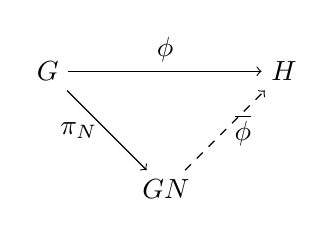
\begin{tikzpicture}
		\node (V) at (0,0) {$G$};
		\node (W) at (3,0) {$H$};
		\node (R) at (1.5,-1.5) {$\lnkset{G}{N}$};
		\draw[->, above] (V) to node {$\phi$} (W);
		\draw[->, left] (V)  to node {$\pi_N$} (R);
		\draw[->, right, dashed] (R)  to node {$\overline{\phi}$} (W);
		\end{tikzpicture}
	\end{center}
\end{proposition}
\begin{proof}
	Existiert so ein $\overline{\phi}$, so ist $\overline{\phi}(gN)=(\overline{\phi}\circ \pi_N)(g)=\phi(g)$ eindeutig bestimmt. Definiere $\overline{\phi}$ nun so.
	\begin{itemize}
		\item $\overline{\phi}$ ist wohldefiniert: $gN = g'N \overset{\propref{1_2_8}}{\Rightarrow}\exists g'=gn$ für ein $n\in N\Rightarrow \phi(g')=\phi(g)\cdot \underbrace{\phi(n)}_{=1}=\phi(g)$, da $n\in\Ker(\phi)$
		\item $\overline{\phi}$ ist Homomorphismus: $\overline{\phi}(gN\cdot g'N) = \overline{\phi}(gg'N)=\phi(gg')=\phi(g)\cdot\phi(g')=\overline{\phi}(gN)\cdot\overline{\phi}(g'N)$
	\end{itemize}
\end{proof}

\begin{conclusion}
	\proplbl{1_3_9}
	Ein Gruppenhomomorphismus $\phi:G\to H$ liefert einen Isomorphismus
	\begin{align}
		\overline{\phi}:\lnkset{G}{\Ker(\phi)}\xrightarrow{\cong}\Image(\phi)\le H\notag
	\end{align}
\end{conclusion}

\begin{conclusion}[1. Homomorphiesatz]
	Seien $H\le G$ und $N\unlhd G$. Der Homomorphismus
	\begin{align}
		\phi: H\overset{i}{\hookrightarrow} HN\xrightarrow{\pi_N}\lnkset{HN}{N}\notag
	\end{align}
	induziert einen Isomorphismus
	\begin{align}
		\overline{\phi}:\lnkset{H}{H\cap N}\xrightarrow{\cong}\lnkset{HN}{N}\notag
	\end{align}
\end{conclusion}
\begin{proof}
	\begin{itemize}
		\item $\phi$ ist surjektiv: Für $h\in H$ und $n\in N$ ist
		\begin{align}
			hnN=hN=\phi(h)\in\phi(H)=\Image(\phi)\notag
		\end{align}
		\item $\Ker(\phi)=H\cap\Ker(\pi_N)=H\cap N$
	\end{itemize}
	Mit \propref{1_3_9} folgt die Behauptung.
\end{proof}

\begin{conclusion}[2. Homomorphiesatz]
	Seien $N\unlhd G$ und $N\le H\unlhd G$. Der Homomorphismus $\pi_H:G\to\lnkset{G}{H}$ induziert einen Isomorphismus
	\begin{align}
		\lnkset{(\lnkset{G}{N})}{(\lnkset{H}{N})}\xrightarrow{\cong}\lnkset{G}{H}\notag
	\end{align}
\end{conclusion}
\begin{proof}
	Da $N\le H$ liefert $\pi_H$ einen Epimorphismus (mit \propref{1_3_8}) $\overline{\pi_H}:\lnkset{G}{N}\to \lnkset{G}{H}$.
	\begin{center}
		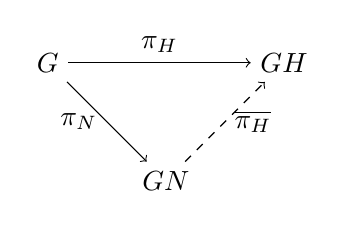
\begin{tikzpicture}
		\node (V) at (0,0) {$G$};
		\node (W) at (3,0) {$\lnkset{G}{H}$};
		\node (R) at (1.5,-1.5) {$\lnkset{G}{N}$};
		\draw[->, above] (V) to node {$\pi_H$} (W);
		\draw[->, left] (V)  to node {$\pi_N$} (R);
		\draw[->, right, dashed] (R)  to node {$\overline{\pi_H}$} (W);
		\end{tikzpicture}
	\end{center}
	Dieser hat Kern $\Ker(\overline{\pi_H})?\lnkset{H}{N}$, induziert nach \propref{1_3_9} einen Isomorphismus
	\begin{align}
		\lnkset{(\lnkset{G}{N})}{\Ker(\overline{\pi_H})}\xrightarrow{\cong}\Image(\overline{\pi_H})=\lnkset{G}{H}\notag
	\end{align}
\end{proof}

\begin{definition}[Konjugation]
	Seien $x,x',g\in G$ und $H,H'\le G$.
	\begin{enumerate}[label=(\alph*)]
		\item $x^g:= g^{-1}xg$, \begriff{Konjugation} von $x$ mit $g$
		\item $x$ und $x'$ sind \begriff{konjugiert} (in $G$)$\Leftrightarrow\exists g\in G$: $x'=x^g$
		\item $H$ und $H'$ heißen \emph{konjugiert} (in $G$)$\Leftrightarrow\exists g\in G$: $H'=H^g=\{h^g\mid h\in H\}$
	\end{enumerate}
\end{definition}

\begin{lemma}
	Die Abbildung
	\begin{align}
		\Int:\begin{cases}
			G\to \Aut(G) \\ g\mapsto (x\mapsto x^g)
		\end{cases}\notag
	\end{align}
	ist ein Gruppenhomomorphismus.
\end{lemma}
\begin{proof}
	\begin{itemize}
		\item $\Int(g)\in\Hom(G,G)$: $(xy)^g=g^{-1}xyg=g^{-1}xgg^{-1}yg=x^g\cdot y^g$
		\item $(x^g)^h=h^{-1}g^{-1}xgh=(gh)^{-1}x(gh)=x^{gh}$
		\item $\Int(g)\in\Aut(G)$: Umkehrabbildung zu $\Int(g)$ ist $\Int(g^{-1})$
		\item $\Int(g)\in\Hom(G,\Aut(G))$:
		\begin{align}
			\Int(gh)=\Int(h)\circ\Int(g)=\Int(g)\cdot\Int(h)\notag
		\end{align}
	\end{itemize}
\end{proof}

\begin{definition}[innere Automorphismen, Zentrum, charakteristische Gruppe]
	\begin{enumerate}[label=(\alph*)]
		\item $\Inn(G)=\Image(\Int)\le\Aut(G)$, die Gruppe der \begriff{inneren Automorphismen} von $G$
		\item $\Z(G)=\Ker(\Int)=\{g\in G\mid xg=gx\quad\forall x\in G\}$, das \begriff{Zentrum} von $G$
		\item $H\le G$ ist \begriff[Gruppe!]{charakteristisch} $\Leftrightarrow\forall\sigma\in\Aut(G)$: $H=H^\sigma$
	\end{enumerate}
\end{definition}

\begin{remark}
	\begin{enumerate}[label=(\alph*)]
		\item Konjugation ist eine Äquivalenzrelation
		\item $H\le G$ ist normal $\Leftrightarrow H=H^\sigma\quad\forall\sigma\in\Inn(G)$
		\item Deshalb gilt für $H\le G$: $H$ ist charakteristisch $\Rightarrow$ $H$ ist normal
	\end{enumerate}
\end{remark}

\begin{example}
	$\Z(G)$ ist charakteristisch in $G$
\end{example}
\section{Abelsche Gruppen}

Sei $G$ ein Gruppe.

\begin{definition}[zyklische Gruppe]
	Eine Gruppe $G$ ist \begriff[Gruppe!]{zyklisch} $\Leftrightarrow G=\langle g\rangle$ für ein $g\in G$.
\end{definition}

\begin{example}
	\begin{enumerate}[label=(\alph*)]
		\item $\whole=\langle 1\rangle$
		\item $\whole/n\whole=\langle\overline{1}\rangle$
		\item $C_n=\langle (1\, 2\, ...\, n)\rangle\le S_n$
		\item Ist $\#G=p$ eine Primzahl, so ist $G$ zyklisch (Übung 6)
	\end{enumerate}
\end{example}

\begin{lemma}
	\proplbl{1_4_3}
	Die Untergruppen von $(\whole,+)$ sind genau die $\langle k\rangle=\whole k$ mit $k\in\natur_0$ und für $k_1,...,k_r\in\whole$ ist $\langle k_1,...,k_r\rangle=\langle k\rangle$ mit
	\begin{align}
		k=\ggT(k_1,...,k_r)\notag
	\end{align}
\end{lemma}
\begin{proof}
	Zwei Beweise sind möglich:
	\begin{enumerate}
		\item Jede Untergruppe von $\whole$ ist ein Ideal von $(\whole,+,\cdot)$ und $\whole$ ist ein Hauptidealring.
		\item Sei $H\le\whole$. Setze $k=\min\{H\cap N\}$, ohne Einschränkung $H\neq\{0\}$.
		\begin{itemize}
			\item $H=\langle k\rangle$: $n\in H\Rightarrow n=qk+r$ mit $q,r\in\whole$, $0\le r<k\Rightarrow r=n-\underbrace{qk}_{k+...+k}\in H\xRightarrow[\text{mal}]{k\text{ mini-}}r=0\Rightarrow n\in\langle k\rangle$
			\item $\langle k_1,...,k_r\rangle=\langle k\rangle\Rightarrow k=\ggT(k_1,...,k_r)$: \\
			$k_i\in\langle k\rangle\Rightarrow k\vert k_i\quad\forall i$ \\
			$k\in\langle k_1,...,k_r\rangle\Rightarrow k=n_1k_1+...+n_rk_r$ mit $n_i\in\whole$ $\exists d\vert k_i\Rightarrow d\vert k\Rightarrow k=\ggT(k_1,...,k_r)$
		\end{itemize}
	\end{enumerate}
\end{proof}

\begin{proposition}[Klassifikation von zyklischen Gruppen]
	Sei $G=\langle g\rangle$ zyklisch. Dann ist $G$ abelsch und
	\begin{enumerate}[label=(\alph*)]
		\item $G\cong (\whole,+)$ \emph{oder}
		\item $G\cong (\whole/n\whole,+)$ mit $n=\#G<\infty$
	\end{enumerate}
\end{proposition}
\begin{proof}
	Betrachte 
	\begin{align}
		\phi: \begin{cases}
		\whole\to G\\ k\mapsto g^k
		\end{cases}\notag
	\end{align}
	$\phi$ ist ein Homomorphismus und surjektiv, da $G=\langle g\rangle$. Nach \propref{1_3_9} ist $G=\Image(\phi)\cong \lnkset{\whole}{\Ker(\phi)}$. Nach \propref{1_4_3} ist $\Ker(\phi)=\langle n\rangle$ für ein $n\in\natur_0$.
	\begin{itemize}
		\item \emph{$n=0$}, so ist $\Ker(\phi)=\langle 0\rangle$, also $\phi$ injektiv und $G\cong\whole$.
		\item \emph{$n>0$}, so ist $G\cong\whole/n\whole$ und $n=\#\whole/n\whole=\#G$.
	\end{itemize}
\end{proof}

\begin{proposition}
	\proplbl{1_4_5}
	Sei $G=(G,+)=\langle g \rangle$ zyklisch der Ordnung $n \in \natur$.
	\begin{enumerate}[label=(\alph*)]
		\item Zu jedem $d \in \natur$ mit $d\mid n$ hat $G$ genau eine Untergruppe der Ordnung $d$, nämlich $U_d=\langle \frac{n}{d}g\rangle$
		\item Für $d \mid n$ und $d'\mid n$ ist $U_d \le U_{d'} \Leftrightarrow d \mid d'$
		\item Für $k_1, \dots , k_k \in \whole$ ist $\langle k_1 g, \dots, k_r g \rangle = \langle eg\rangle = U_{\sfrac{n}{e}}$ mit $e = \ggT(k_1,\dots,k_r,n)$
		\item Für $k \in \whole$ ist $\ord(kg)= \frac{n}{\ggT(k,n)}$
	\end{enumerate}
\end{proposition}
\begin{proof}
	Betrachte wieder 
	\begin{align}
		\phi: \begin{cases}\overline{k} \to G \\k \mapsto kg\end{cases}\notag
	\end{align}
	\begin{enumerate}[label=(\alph*)]
		\item Nach \propref{1_3_7} und \propref{1_4_3} liefert $\phi$ Bijektion 
		\begin{align}
			\{ e \in \natur \mid n\whole \le e\whole \} \xrightarrow{\propref{1_1_1}} \{ H \le G \}\notag
		\end{align}
		 und $n\whole \le e\whole \Leftrightarrow e \mid n$. Ist $H = \phi(e\whole) = \langle eg \rangle$, so ist $H \cong \lnkset{e\whole}{n\whole}$, also $n = (\whole :  n \whole) = (\whole : e\whole)\cdot(e\whole : n\whole) = e \cdot \#H$
		\item $U_d \le U_{d'} \Leftrightarrow \langle \frac{n}{d}g \rangle \le \langle \frac{n}{d'}g \rangle \Leftrightarrow \frac{n}{d}\whole \le \frac{n}{d'}\whole \Leftrightarrow \frac{n}{d'} \mid \frac{n}{d} \Leftrightarrow d \mid d'$
		\item Mit $H = \langle k_1, \dots, k_r,n \rangle \le \whole$ ist $n\whole \le H$, $\phi(H) = \langle k_1 g, \dots, k_r g\rangle$. Nach \propref{1_4_3} ist $H = \langle e \rangle$ mit $e = \ggT(k_1, \dots, k_r, n)$, somit $\langle k_1 g, \dots, k_r g \rangle = \phi(e\whole) = U_{\sfrac{n}{e}}$
		\item $\ord(kg) = \#\langle kg \rangle \overset{c)}{=} \#U_{\sfrac{n}{e}}$ mit $e = \ggT(k,n)$
	\end{enumerate}
\end{proof}

\begin{lemma}
	\proplbl{1_4_6}
	Seien $a,b \in G$. Kommutieren $a$ und $b$ und sind $\ord(a)$ und $\ord(b)$ teilerfremd, so ist
	\begin{align}
		\ord(a,b) = \ord(a)\cdot \ord(b) \notag
	\end{align}
\end{lemma}
\begin{proof}
	Nach \propref{1_2_12} ist $\langle a \rangle \cap \langle b \rangle = 1$. Ist $(ab)^k = 1 = a^k b^k$, so ist $a^k = b^{-k} \in \langle a \rangle \cap \langle b \rangle = 1$, also $a^k = b^k = 1$. Somit ist $(ab)^k = 1 \Leftrightarrow a^k = 1$ und $b^k =1$ und damit $\ord(ab) = \kgV(\ord(a), \ord(b)) = \ord(a) \cdot \ord(b)$
\end{proof}

\begin{conclusion}
	\proplbl{1_4_7}
	Ist $G$ abelsch und sind $a,b \in G$ mit $\ord(a) = m < \infty$, $\ord(b) = n < \infty$, so existiert $c \in G$ mit
	\begin{align}
		\ord(c) = \kgV(\ord(a), \ord(b)) \notag
	\end{align}
\end{conclusion}
\begin{proof}
	Schreibe $m = m_0 m'$ und $n = n_0 n'$ mit $m_0 n_0 = \kgV(m,n)$ und $\ggT(m_0, n_0) = 1 \Rightarrow \ord(a^{m'}) = m_0$, $\ord(b^{n'}) = n_0 \Rightarrow \ord(b^{n'} \cdot a^{m'}) \overset{\propref{1_4_6}}{=} m_0 \cdot n_0 = \kgV(m,n)$.
\end{proof}

\begin{theorem}[Struktursatz für endlich erzeugte abelsche Gruppen]
	\proplbl{1_4_8}
	Jede endliche erzeugte abelsche Gruppe $G$ ist eine direkte Summe zyklischer Gruppen
	\begin{align}
		G \cong \whole^{r} \oplus\bigoplus_{i=1}^k \lnkset{\whole}{d_i \whole} \notag
	\end{align}
	mit eindeutig bestimmten $d_1, \dots, d_k > 1$ die $d_i \mid d_{i+1}$ für alle $i$ erfüllen.
\end{theorem}
\begin{proof}
	\begin{itemize}
		\item Existenz: LAAG 2: VIII. 6.14
		\item Eindeutigkeit: Für $d \in \natur$ ist 
		\begin{align}
			\# \lnkset{G}{dG} &= \#\left( \lnkset{\whole}{d \whole}\right)^r \oplus \bigoplus_{i=1}^k \lnkset{\left(\lnkset{\whole}{d_i\whole}\right)}{d\cdot\left(\lnkset{\whole}{d_i\whole}\right)} \notag \\
			&\overset{\propref{1_4_5}}{=} d^r \cdot \prod_{i=1}^{n} \frac{d_i}{\ggT(d,d_i)}\notag
		\end{align} 
	\end{itemize}
und daraus kann man $r, k, d_1, \dots , d_k$ erhalten.
\end{proof}

\begin{lemma}
	Sei $G=(G,+) = \langle g\rangle$ zyklisch der Ordnung $n \in \natur$. Die Endomorphismen von $G$ sind genau die 
	\begin{align}
		\phi_{\overline{k}}: \begin{cases}
		G \to G \\
		x \mapsto kx
		\end{cases} \text{ für } \overline{k} = k + n\whole \in \whole/n\whole\notag
	\end{align}
	Dabei ist $\phi_{\overline{l}}\circ\phi_{\overline{k}} = \phi_{\overline{kl}}$.
\end{lemma}
\begin{proof}
	\begin{itemize}
		\item $\phi_{\overline{k}}$ wohldefiniert $\overline{k_1} = \overline{k_2} \Rightarrow k_2 = k_1 +an$ mit $a \in \whole\Rightarrow k_2 x = k_1 x + a n \cdot x$, aber $nx=0$.
		\item $\phi_{\overline{k}} \in \Hom(G,G)$: klar, da $G$ abelsch
		\item $\overline{k}=\overline{l}\Leftrightarrow \phi_{\overline{k}} = \phi_{\overline{l}}$: $\phi_{\overline{k}}(g) = \phi_{\overline{l}}(g) \Rightarrow (k-l)g = 0 \xRightarrow[=n]{\ord(g)} n \mid (k-l) \Rightarrow \overline{k} = \overline{l}$
		\item $\phi \in \Hom(G,G) \Rightarrow \phi = \phi_{\overline{k}}$ für ein $k \in \whole$: $\phi(g) = kg$ für ein $k \Rightarrow \phi = \phi_{\overline{k}}$
		\item $\phi_{\overline{k}} \circ \phi_{\overline{l}} = \phi_{\overline{kl}}$: $l(kx) = (lk)x$
	\end{itemize}
\end{proof}

\begin{proposition}
	Ist $G$ zyklisch von Ordnung $n \in \natur$, so ist
	\begin{align}
		\Aut(G) \cong (\whole/n\whole)^{\times}\notag
	\end{align}
\end{proposition}
\begin{proof}
	$\Aut(G) \subseteq \Hom(G,G) = \{ \phi_{\overline{k}} \mid \overline{k} \in \whole/n\whole\}$, $\phi_{\overline{k}}\in\Aut(G)\Leftrightarrow$ es existiert ein $\overline{l}\in\whole/n\whole$ mit $\phi_{\overline{l}}\circ\phi_{\overline{k}}=\phi_{\overline{1}}$ also existiert ein $\overline{l}\in\whole/n\whole$ mit $\overline{kl}=1\Leftrightarrow\overline{k}\in (\whole/n\whole)^\times$ und 
	\begin{align}
		\begin{cases}
		(\whole/n\whole)^\times&\to \Aut(G) \\
		\overline{k}&\mapsto \phi_{\overline{k}}
		\end{cases}\notag
	\end{align}
	ist ein Isomorphismus.
\end{proof}

\begin{definition}[\person{Euler}'sche Phi-Funktion]
	\begin{align}
		\Phi(n) = \#(\whole/n\whole)^\times\notag
	\end{align}
	ist die \begriff{\person{Euler}'sche Phi-Funktion}.
\end{definition}

\begin{example}
	$p$ prim $\Rightarrow$ $\phi(p) = p-1$, da $\whole / p\whole$ Körper ist.
\end{example}

\begin{proposition}
	Ist $K$ ein Körper und $H\leq K^{\times}$ abelsch, so ist $H$ zyklisch.
\end{proposition}
\begin{proof}
	Setze $m=\max\{\ord(h) \colon h \in H\}$. Nach \propref{1_4_7} gilt $\ord(h) \mid m \quad\forall h \in H$. $\Rightarrow$ Jedes $h \in H$ ist Nullstelle von $f = x^m -1 \in K[x]$. $\Rightarrow$ $\# H \leq \deg f = m \leq \# H \Rightarrow \# H = m$. Ist $h \in H$ mit $m = \ord(h)$, so ist dann $H = \langle h \rangle$.
\end{proof}

\begin{conclusion}
	\proplbl{1_4_14}
	Für $p \in \natur$ prim ist
	\begin{align}
		\Aut(C_p) \cong (\whole / p \whole)^{\times} \cong C_{p-1}\notag
	\end{align}
\end{conclusion}
\section{Direkte und semidirekte Produkte}

Sei $G$ eine Gruppe und $n\in\natur$.

\begin{definition}[direktes Produkt]
	Das \begriff{direkte Produkt} von Gruppen $G_1,...,G_n$ ist das kartesische Produkt
	\begin{align}
		G=\prod_{i=1}^n G_1 = G_1\times ...\times G_n=\bigtimes_{i=1}^n G_1\notag
	\end{align}
	mit komponentenweiser Multiplikation.
\end{definition}

\begin{remark}
	\begin{enumerate}[label=(\alph*)]
		\item Wir identifizieren $G_j$ mit der Untergruppe
		\begin{align}
			G_j = \prod_{i\neq j} 1 = 1\times ...\times 1\times G_j\times 1 \times ...\times 1\notag
		\end{align}
		von $\prod_{i=1}^n G_j$.
		\item Für $i\neq j$, $g_i\in G_i$, $g_j\in G_j$ gilt dann
		\begin{align}
			\label{1.1}
			g_ig_j=g_jg_i
		\end{align}
	\end{enumerate}
\end{remark}

\begin{definition}[internes direktes Produkt]
	Seien $H_1,...,H_n\le G$. Dann ist $G$ das \begriff{interne direkte Produkt} von $H_1,...,H_n$, in Zeichen
	\begin{align}
		G = \prod_{i=1}^n H_i = H_1\times ...\times H_n=\bigtimes_{i=1}^n H_i\notag
	\end{align} 
	wenn
	\begin{align}
		\begin{cases}
		H_1\times ...\times H_n &\to G \\
		(g_1,...,g_n) &\mapsto g_1\cdot ...\cdot g_n
		\end{cases}\notag
	\end{align}
	ein Gruppenisomorphismus ist.
\end{definition}

\begin{proposition}
	\proplbl{1_5_4}
	Seien $U,V\le G$. Dann sind äquivalent:
	\begin{enumerate}[label=(\roman*)]
		\item $G=U\times V$
		\item $U\unlhd G$, $V\unlhd G$, $U\cap V=1$, $UV=G$
	\end{enumerate}
\end{proposition}
\begin{proof}
	\begin{itemize}
		\item $(i)\Rightarrow (ii)$: Im externen direkten Produkt $U\times V$ gilt:
		\begin{itemize}
			\item $UV=U\times V$: Für $u\in U$, $v\in V$ ist $(u,v)=(u,1)\cdot (1,v)\in UV$
			\item $U\cap V=1$: klar
			\item $U\unlhd U\times V$: Für $g=(u,v)\in U\times V$ und $u_0=(u_0,1)\in U$ ist 
			\begin{align}
				u_0^g = g^{-1}u_0g=(u^{-1},v^{-1})(u_0,1)(u,v)=(u_0^u,1)\in U\notag
			\end{align}
		\end{itemize}
		\item $(ii)\Rightarrow (i)$: betrachte 
		\begin{align}
			\phi: \begin{cases}
			U\times V\to G \\ (u,v)\mapsto w
			\end{cases}\notag
		\end{align}
		\begin{itemize}
			\item \cref{1.1} gilt: Für $u\in U$, $v\in V$ gilt in $G$:
			\begin{align}
				u^{-1}v^{-1}uv=\underbrace{(v^{-1})^uv}_{\in V} = \underbrace{u^{-1}u^v}_{\in U}\cap V=1\Rightarrow uv=vu\notag
			\end{align}
			\item $\phi$ ist Homomorphismus: $\phi((u_1,v_1)(u_2,v_2)) = \phi(u_1u_2,v_1v_2) = u_1u_2v_1v2 \overset{\eqref{1.1}}{=} u_1v_1u_2v_2 = \phi(u_1,v_1)\cdot \phi(u_2,v_2)$
			\item $\phi$ surjektiv: $\Image(\phi)=UV=G$
			\item $\phi$ injektiv: $1=\phi(u,v) = uv\Rightarrow u=v^{-1}\in U\cap V = 1\Rightarrow (u,v) = (1,1)$
		\end{itemize}
	\end{itemize}
\end{proof}

\begin{conclusion}
	Seien $H_1,...,H_n\le G$. Dann sind äquivalent:
	\begin{enumerate}[label=(\roman*)]
		\item $G=H_1\times ...\times H_n$
		\item $G=H_1...H_n$ und $\forall i$: $H_i\unlhd G$ und $H_{i-1}\cap H_i=1$
	\end{enumerate}
\end{conclusion}
\begin{proof}
	Induktion nach $n$. \\
	\emph{$n=1$:} trivial \\
	\emph{$n>1$:} Setze $U=H_1...H_{n-1}$ und $V=H_n$. Dann ist $U\unlhd G$ (\propref{1_3_3} c) und $V\unlhd G$, $UV=H_1...H_n=G$, $U\cap V=1$. Somit ist $\phi: U\times V\to G$ ein Isomorphismus nach \propref{1_5_4}. Da $H_i\unlhd U$ für $i<n$ folgt nach Induktionshypothese, dass
	\begin{align}
		\phi':\begin{cases}
		H_1...H_{n-1} &\to U \\ (h_1,...,h_{n-1}) &\mapsto h_1...h_{n-1}
		\end{cases}\notag
	\end{align}
	Somit ist 
	\begin{align}
		\phi\circ (\phi'\times \id_{H_n}):\begin{cases}
		H_1...H_n &\to G \\ (h_1...h_n) &\mapsto \phi(\phi'((h_1,...,h_{n-1}),h))=h_1...h_n
		\end{cases}\notag
	\end{align}
	ein Isomorphismus.
\end{proof}

\begin{definition}[internes semidirektes Produkt]
	Seien $H,N\le G$. Dann ist $G$ das \begriff{interne semidirekte Produkt} von $H$ und $N$, in Zeichen
	\begin{align}
		G=H\ltimes N = N\rtimes H\notag
	\end{align}
	wenn $N\unlhd G$, $H\cap N=1$ und $NH=G$.
\end{definition}

\begin{remark}
	\proplbl{1_5_7}
	Ist $G=H \ltimes N$, so ist
	\begin{align}
		\alpha: \begin{cases}
		H\to \Aut(N) \\ h \mapsto \Int(h)\vert_N
		\end{cases}\notag
	\end{align}
	ein Gruppenhomomorphismus. Im Fall $G=H\times N$ ist $\alpha(h)=\id_N$ für alle $h\in H$. Für $h_1,h_2\in H$ und $n_1,n_2\in N$ ist
	\begin{align}
		h_1n_1\cdot h_2n_2 &= h_1h_2h_2^{-1}n_1h_2n_2 \notag \\
		&= h_1h_2\cdot \underbrace{n_1^{h_2}}_{\in N}\cdot n_2 \notag \\
		\label{1.2}
		&= h_1h_2\cdot n_1^{\alpha(h_2)}\cdot n_2
	\end{align}
\end{remark}

\begin{definition}[semidirektes Produkt]
	Seien $H,N$ Gruppen und $\alpha\in\Hom(H,\Aut(N))$. Das \begriff{semidirekte Produkt} $H\ltimes_{\alpha}N$ von $H$ und $N$ bezüglich $\alpha$ ist das kartesische Produkt $H\times N$ mit der Multiplikation
	\begin{align}
		(h_1,n_1)\cdot (h_2,n_2) = (h_1h_2,n_1^{\alpha(h_2)}n_2)\notag
	\end{align}
\end{definition}

\begin{remark}
	\begin{enumerate}[label=(\alph*)]
		\item Wir identifizieren $H,N$ mit der Teilmenge $H\times 1$ bzw. $N\times 1$ von $H\ltimes_{\alpha} N$.
		\item Ist $\alpha\in\Hom(H,\Aut(N))$ trivial, also $\alpha(h)=\id_N$ für alle $h\in H$, so ist $H\ltimes_{\alpha} N=H \times N$, das direkte Produkt.
	\end{enumerate}
\end{remark}

\begin{proposition}
	Seien $H,N$ Gruppen, $\alpha\in\Hom(H,\Aut(N))$. Dann ist $G=H\ltimes_{\alpha} N$ eine Gruppe, und diese ist das interne semidirekte Produkt von $H\le G$ und $N\unlhd G$, wobei
	\begin{align}
		\Int(h)\vert_N = \alpha(h)\quad\forall h\in H\notag
	\end{align}
\end{proposition}
\begin{proof}
	Seien $h_1$, $h_2$, $h_3$, $h\in H$ und $n_0$, $n_1$, $n_2$, $n_3$, $n\in N$.
	\begin{itemize}
		\item neutrales Element: 
		\begin{align}
			(1_H,1_N)(h,n) &= (h,1_N^{\alpha(h)}n) = (h,n) \notag \\
			(h,n)(1_H,1_N) &= (h,n^{\alpha(1_H)}1_H) \overset{(\ast)}{=} (h,n) \notag
		\end{align}
		$(\ast)$: $\alpha(1_H)=\id$
		\item Assoziativität:
		\begin{align}
			[(h_1,n_1)(h_2,n_2)](h_3,n_3) &= (h_1h_2,n_1^{\alpha(h_2)}n_2)(h_3,n_3) = (h_1h_2h_3,(n_1^{\alpha(h_2)}n_2)^{\alpha(h_3)}n_3) \overset{(\ast)}{=} (h_1h_2h_3,n_1^{\alpha(h_2)\alpha(3)}n_2^{\alpha(h_3)}n_3) \notag \\
			(h_1,n_1)[(h_2,n_2)(h_3,n_3)] &= (h_1,n_1)(h_2h_2,n_2^{\alpha(h_3)}n_3) = (h_1h_2h_3,n_1^{\alpha(h_2)\alpha(3)}n_2^{\alpha(h_3)}n_3) \notag
		\end{align}
		$(\ast)$: $\alpha(h_3)$ ist ein Automorphismus und $\alpha$ ist ein Homomorphismus
		\item Inverses: $(h,n)^{-1}=(h^{-1},(n^{-1})^{\alpha(h^{-1})})$
		\item $H\le G$:
		\begin{align}
			(h_1,1)(h_2,1) &= (h_1h_2,1^{\alpha(h_2)}1) = (h_1h_2,1)\in H \notag \\
			(h,1)^{-1} &= (h^{-1},1)\in H \notag
		\end{align}
		\item $N\le G$:
		\begin{align}
			(1,n_1)(1,n_2) &= (1,n_1^{\alpha(1)}n_2) = (1,n_1n_2)\in N \notag \\
			(1,n)^{-1} &= (1,(n^{-1})^{\alpha(1^{-1})}) = (1,n^{-1})\in N \notag
		\end{align}
		\item $H\cap N=1$: klar
		\item $HN=G$: $(h,1)(1,n)=(h,1^{\alpha(1)}n)=(h,n)\in G$
		\item $N\unlhd G$: $(h,n)^{-1}(1,n_0)(h,n)=(h^{-1},(n^{-1})^{\alpha(h^{-1})})(h,n_0^{\alpha(h)}n)=(1,...)\in N$
		\item $\Int(h)\vert_N=\alpha(h)$:
		\begin{align}
			n^{\Int(h)\vert_N} &= (h,1)^{-1} (1,n)(h,1) \notag \\
			&= (h^{-1},1)(h,n^{\alpha(h)}1) \notag \\
			&= (1,1^{\alpha(h)}n^{\alpha(h)}) \notag \\
			&= (1,n^{\alpha(h)}) \notag \\
			&= n^{\alpha(h)} \notag
		\end{align}
	\end{itemize}
\end{proof}

\begin{conclusion}
	Sei $G=H\ltimes N$ und $\alpha$ wie in\propref{1_5_7}. Dann ist
	\begin{align}
		\phi :\begin{cases}
		H\ltimes_{\alpha} N &\to G \\ (h,n) &\mapsto hn
		\end{cases}\notag
	\end{align}
	ein Isomorphismus. Insbesondere ist $G$ durch $H$, $N$ und $\alpha$ bis auf Isomorphie eindeutig bestimmt.
\end{conclusion}
\begin{proof}
	\begin{itemize}
		\item $\phi$ ist Homomorphismus: $\phi((h_1,n_1)\cdot (h_2,n_2)) = \phi(h_1h_2,n_1^{\alpha(h_2)}n_2) = h_1h_2n_1^{\alpha(h_2)}n_2 \overset{\eqref{1.2}}{=} h_1h_2n_1n_2 = \phi(h_1,n_1)\cdot \phi(h_2,n_2)$
		\item $\phi$ ist surjektiv: $\Image(\phi)=HN=G$
		\item $\phi$ ist injektiv: $H\cap N=1$
	\end{itemize}
\end{proof}

\begin{example}
	Sei $G=H\ltimes N$.
	\begin{enumerate}[label=(\alph*)]
		\item $H=N=C_2$: $\Aut(N)=\{\id_{C_2}\}\Rightarrow\alpha\in\Hom(C_2,\Aut(C_2))=1$ (konstante Abbildung) $\Rightarrow G = H\ltimes_{\alpha} N=H\times N\cong C_2\times C_2\cong V_4$
		\item $H=C_2$, $N=C_3$: $\Aut(N)\cong (\whole/3\whole)^\times\cong C_2 \Rightarrow \alpha\in\Hom(C_2,\Aut(C_3))=\{\id_{C_2}, 1\}\Rightarrow H\ltimes_{\alpha} N = H\times N\cong C_6$ oder $H\ltimes_{\id_{C_2}}N\cong S_3$
	\end{enumerate}
\end{example}

\section{Gruppenwirkungen}

Sei $G$ eine Gruppe und $X$ eine Menge.

\begin{definition}[Wirkung, $G$-Menge]
	Eine (rechts-)\begriff{Wirkung} von $G$ auf $X$ ist eine Abbildung
	\begin{align}
		\begin{cases}
			X\times G\to X \\ (x,g)\mapsto x^g
		\end{cases}\notag
	\end{align}
	mit $x\in X$ und $h,g\in G$, wobei
	\begin{itemize}
		\item (W1): $x^{1_G}=x$
		\item (W2): $(x^g)^h=x^{gh}$
	\end{itemize}
	Eine \begriff{$G$-Menge} ist eine Menge $X$ zusammen mit einer Wirkung von $G$ auf $X$.
\end{definition}

\begin{example}
	\proplbl{1_6_2}
	\begin{enumerate}[label=(\alph*)]
		\item Die symmetrische Gruppe $G=\Sym(X)$ wirkt auf $X$ durch $x^\sigma=\sigma(x)$ mit $x\in X$, $\sigma\in G$. So wirkt zum Beispiel $S_n$ auf $X=\{1,...,n\}$.
		\item $G$ wirkt auf $X=G$ durch Multiplikation $x^g=xg$, die sogenannte \begriff{reguläre Darstellung} von $G$.
		\item $G$ wirkt auf $X=G$ durch Konjugation: $x^g=g^{-1}xg$.
		\item $G$ wirkt auf der Menge $\UG(G)$ der Untergruppen von $G$ durch Konjugation $H^g=\{h^g\mid h\in H\}$ mit $H\le G$.
		\item Sind $H,N$ Gruppen, so liefert jedes $\alpha\in\Hom(H,\Aut(N))$ eine Wirkung von $H$ auf $N$ durch $n^h=n^{\alpha(h)}$.
		\item Ist $K$ ein Körper, so wirkt $K^\times$ auf $K$ durch $x^y=xy$ mit $x\in K$ und $y\in K^\times$.
		\item Ist $K$ ein Körper, $n\in\natur$, so wirkt $\GL_n(K)^{op}$ auf $K^n$ durch Multiplikation $x^A=Ax$
	\end{enumerate}
\end{example}

\begin{*anmerkung}
	$^{op}$ ist nötig, weil die Multiplikation "'falsch herum"' definiert wurde. g) wäre ein Beispiel für eine Linkswirkung, also ist es dann mit $^{op}$ eine Rechtswirkung.
\end{*anmerkung}

\begin{*example}
	The additive group of the real numbers $(\real, +)$ acts on the phase space $V = \real^3$ of ``well-behaved'' systems in classical mechanics (and in more general dynamical systems) by time translation: if $t$ is in $\real$ and $x$ is in the phase space, then $x$ describes a state of the system, and $t + x$ is defined to be the state of the system $t$ seconds later if $t$ is positive or $-t$ seconds ago if $t$ is negative.
\end{*example}

\begin{remark}
	\proplbl{1_6_3}
	Wirkt $G$ auf $X$, so ist für jedes $g\in G$ die Abbildung
	\begin{align}
		\sigma_g: \begin{cases}
			X\to X \\ x\mapsto x^g
		\end{cases} \notag
	\end{align}
	bijektiv, da $\sigma_g\circ\sigma_{g^{-1}}=\sigma_{g^{-1}}\sigma_g=\sigma_1=\id_X$, also $\sigma_g\in\Sym(X)$ und
	\begin{align}
		\begin{cases}
			G\to \Sym(G) \\ g\mapsto \sigma_g
		\end{cases}\notag
	\end{align}
	ist ein Gruppenhomomorphismus. Umgekehrt liefert jeder Homomorphismus $\sigma: G\to\Sym(G)$ eine Wirkung von $G$ auf $X$ durch $x^g=x^{\sigma(g)}$. Somit steht die Menge der Wirkungen von $G$ auf $X$ in natürlicher Bijektion zu $\Hom(G,\Sym(X))$.
\end{remark}

\begin{definition}[Fixpunkt, Stabilisator, Bahn, Bahnraum, $G$-invariant, treu, transitiv, frei]
	Sei $X$ eine $G$-Menge, $g_0\in G$, $x_0\in X$
	\begin{enumerate}[label=(\alph*)]
		\item $x_0$ ist ein \begriff{Fixpunkt} von $g_0\Leftrightarrow x_0^{g_0}=x_0$
		\item $\Fix(G) = X^G = \{x\in X\mid x^g=x\quad\forall g\in G\}$, die Menge der Fixpunkte von $X$ unter $G$
		\item $G_{x_0} = \Stab(x_0) = \{g\in G\mid x_0^g = x\}$ der \begriff{Stabilisator} von $x_0$ in $G$
		\item $x_0^G = \{x_0^g \mid g\in G\}$, die \begriff{Bahn} von $x_0$ unter G
		\item $\lnkset{X}{G} = \{x^G\mid x\in X\}$, der \begriff{Bahnenraum}
		\item $Y\le X$ ist \begriff{$G$-invariant} $\Leftrightarrow Y^g = \{y^g\mid y\in Y\}\le Y$
		\item Die Wirkung von $G$ auf $X$ ist
		\begin{itemize}
			\item \begriff{treu}, wenn $\bigcap_{x\in X} G_x=1$
			\item \begriff{transitiv}, wenn gilt: $\forall x,y\in X\exists g\in G$: $x^g=y$
			\item \begriff{frei}, wenn $G_x=1$ für alle $x\in X$
		\end{itemize}
	\end{enumerate}
\end{definition}

\begin{remark}
	\begin{enumerate}[label=(\alph*)]
		\item Der Stabilisator $G_{x_0}$ besteht aus den $g\in G$, die $x_0$ als Fixpunkt haben.
		\item Die Wirkung von $G$ auf $X$ ist
		\begin{itemize}
			\item transitiv, wenn es nur eine Bahn gibt, also $\vert\lnkset{X}{G}\vert = 1$
			\item frei, wenn kein $1\neq g\in G$ einen Fixpunkt hat
			\item treu, wenn kein $1\neq g\in G$ alle $x\in X$ als fixiert
		\end{itemize}
	\end{enumerate}
\end{remark}

\begin{example}
	Für $n>1$ wirkt $G=S_n$ auf $X=\{1,...,n\}$ transitiv, treu, aber für $n\ge 3$ nicht frei. Der Stabilisator $G_n$ von $n\in X$ ist eine Untergruppe von $S_n$ isomorph zu $S_{n-1}$.
\end{example}

\begin{example}
	\proplbl{1_6_7}
	Die reguläre Darstellung von $G$ auf $X=G$ ist frei und transitiv:
	\begin{itemize}
		\item frei: $x^g=x\Rightarrow xg=x\Rightarrow g=1$
		\item transitiv: $x,y\in X=G\Rightarrow$ für $g=x^{-1}y$ ist $x^g=y$
	\end{itemize}
\end{example}

\begin{lemma}
	\proplbl{1_6_8}
	Sei $X$ eine $G$-Menge.
	\begin{enumerate}[label=(\alph*)]
		\item Für $x\in X$ ist $G_x\le G$.
		\item Für $x,y\in X$ ist $x^G=y^G$ oder $x^G\cap y^G=\emptyset$.
		\item $\bigcap_{x\in X}=\Ker(\sigma)$, $\sigma:G\to\Sym(X)$ wie in \propref{1_6_3}
		\item Für $x\in X$ und $g\in G$ ist $G_{x^g}=(G_x)^g$
	\end{enumerate}
\end{lemma}
\begin{proof}
	Seien $x,y\in X$, $g,h\in G$
	\begin{enumerate}[label=(\alph*)]
		\item Sei $x^g=x$ und $x^h=x$. Dann
		\begin{align}
			x^{g^h}&=(x^g)^h=x^h=x\Rightarrow gh\in G_x \notag \\
			x^{g^{-1}} &= (x^g)^{g^{-1}} = x^1 = x\RightTorque g^{-1}\in G_x \notag
		\end{align}
		\item $x^g=y^h\Rightarrow x^G=(x^g)^G=(y^h)^H=y^H$
		\item $g\in\bigcap_{x\in X} G_x\Rightarrow\forall x\in X$: $x^g=x\Leftrightarrow \sigma_g=\sigma(g)\id_X$
		\item $h\in G_{x^g}\Leftrightarrow (x^g)^h=x^g\Leftrightarrow x^{ghg^{-1}}=x\Leftrightarrow h^{g^{-1}}\in G_x\Leftrightarrow h\in (G_x)^g$
	\end{enumerate}
\end{proof}

\begin{proposition}[\person{Cayley}]
	Ist $n=\#G<\infty$, so ist $G$ isomorph zu einer Untergruppe der $S_n$.
\end{proposition}
\begin{proof}
	Betrachte die reguläre Darstellung $\sigma:G\to\Sym(G)$. Da diese Wirkung frei ist (\propref{1_6_7}), also insbesondere treu, ist $\sigma$ injektiv (\propref{1_6_8} c), somit $G\cong \Image(\sigma)\le\Sym(G)$. Eine Aufzählung $G=\{g_1,...,g_n\}$ liefert einen Isomorphismus
	\begin{align}
		\phi:\begin{cases}
			S_n\to \Sym(X) \\ \tau\mapsto (g_i\mapsto g_{\tau(i)})
		\end{cases}\notag
	\end{align}
	und somit ist $G\cong \phi^{-1}(\Image(\sigma))\le S_n$.
\end{proof}

\begin{lemma}
	\proplbl{1_6_10}
	Für eine $G$-Menge $X$ und $x\in X$ ist
	\begin{align}
		\phi:\begin{cases}
			\rnkset{G}{G_x}\to x^G \\ G_xg\mapsto x^g
		\end{cases}\notag
	\end{align}
	eine Bijektion.
\end{lemma}
\begin{proof}
	\begin{itemize}
		\item $\phi$ wohldefiniert: $G_xg=G_xg'\Rightarrow g'=gh$ mit $h\in G_x\Rightarrow x^{g'}=x^{hg}=x^g$
		\item $\phi$ surjektiv: klar
		\item $\phi$ injektiv: $x^g=x^{g'}\Leftrightarrow x=x^{g'g^{-1}}\Leftrightarrow g'g^{-1}\in G_x\Leftrightarrow g'\in G_xg\Leftrightarrow Gx_g'=G_xg$
	\end{itemize}
\end{proof}

\begin{proposition}[Bahn-Stabilisator-Satz]
	\proplbl{1_6_11}
	Sei $X$ eine $G$-Menge, $x\in X$. Dann ist
	\begin{align}
		\# x^G = (G:G_x) \notag
	\end{align}
\end{proposition}
\begin{proof}
	\propref{1_6_10}
\end{proof}

\begin{*example}
	Da bei Prof Fehm, die Verbindung zwischen Algebra und Geometrie keine Beachtung geschenkt wird, hier mal ein sehr anschauliches Beispiel von Wikipedia.\\
	One can use the orbit-stabilizer theorem \propref{1_6_11} to count the automorphisms of a graph. Consider the cubical graph, and let $G$ denote its automorphism group. Then G acts on the set of vertices $\{1,2,\dots,8\}$, and this action is transitive as can be seen by composing rotations about the center of the cube. Thus, by the orbit-stabilizer theorem, we have that $|G|=|G\cdot 1||G_{1}|=8|G_{1}|$. Applying the theorem now to the stabilizer $G_{1}$, we obtain $|G_{1}|=|(G_{1})\cdot 2||(G_{1})_{2}|$ . Any element of $G$ that fixes $1$ must send $2$ to either $2$, $4$ or $5$. There are such automorphisms; consider for example the map that transposes $2$ and $4$, transposes $6$ and $8$, and fixes the other vertices. Thus, $\left|(G_{1})\cdot 2\right|=3$. Applying the theorem a third time gives $|(G_{1})_{2}|=|((G_{1})_{2})\cdot 3||((G_{1})_{2})_{3}|$. Any element of $G$ that fixes $1$ and $2$ must send $3$ to either $3$ or $6$, and one easily finds such automorphisms. Thus, $\left|((G_{1})_{2})\cdot 3\right|=2$. One also sees that $((G_{1})_{2})_{3}$ consists only of the identity automorphism, as any element of $G$ fixing $1$, $2$ and $3$ must also fix $4$ and consequently all other vertices. Combining the preceding calculations, we now obtain $|G|=8\cdot 3\cdot 2\cdot 1=48$. 
	% https://en.wikipedia.org/wiki/Group_action#Orbit-stabilizer_theorem_and_Burnside's_lemma 
\end{*example}

\begin{conclusion}[Bahngleichung]
	Ist $X$ eine $G$-Menge und $X=\biguplus_{i=1}^n x_i^G$ die Zerlegung von $X$ in Bahnen (vgl. \propref{1_6_8} c) so ist
	\begin{align}
		\# X= \sum_{i=1}^{n} (G:G_i)\notag
	\end{align}
\end{conclusion}

\begin{definition}[Zentralisator, Normalisator]
	\begin{enumerate}[label=(\alph*)]
		\item Für $h\in H$ ist 
		\begin{align}
			C_G(h) = \{g\in G\mid gh=hg\}\notag
		\end{align}
		der \begriff{Zentralisator} von $h$.
		\item Für $H\le G$ ist 
		\begin{align}
		N_G(h) = \{g\in G\mid gH=Hg\}\notag
		\end{align}
		der \begriff{Normalisator} von $H$.
	\end{enumerate}
\end{definition}

\begin{remark}
	\begin{enumerate}[label=(\alph*)]
		\item Der Zentralisator von $h$ ist der Stabilisator von $h$ unter der Wirkung von $G$ auf $X=G$ durch Konjugation (\propref{1_6_2} c). Es ist die größte Untergruppe $H$ mit $h\in \Z(h)$.
		\item Der Normalisator von $H\le G$ ist der Stabilisator von $H$ unter der Wirkung von $G$ auf $X=\UG(G)$ durch Konjugation (\propref{1_6_2} d). Dies ist die größte Untergruppe $N$ von $G$ mit $H\unlhd N$.
	\end{enumerate}
\end{remark}

\begin{conclusion}
	\proplbl{1_6_15}
	Für $h\in G$ und $H\le G$ ist $C_G(h)\le G$ und $H\unlhd N_G(H)\le G$ und 
	\begin{enumerate}[label=(\alph*)]
		\item $(G:C_G(h))$ ist genau die Anzahl der zu $h$ konjugierten Elemente von $G$
		\item $(G:N_G(H))$ ist genau die Anzahl der zu $H$ konjugierten Untergruppen von $G$
	\end{enumerate}
\end{conclusion}
\begin{proof}
	\propref{1_6_11}
\end{proof}

\begin{conclusion}[Klassengleichung]
	\proplbl{1_6_16}
	Sei $G$ endlich mit Zentrum $Z=\Z(G)$ und sei $x_1,...,x_n$ ein Repräsentantensystem der Konjugationsklassen in $G\setminus Z$. Dann ist
	\begin{align}
		\#G = \#Z + \sum_{i=1}^n (G:C_G(x_i))\notag
	\end{align}
\end{conclusion}
\begin{proof}
	aus \propref{1_6_11} und \propref{1_6_15}, da $G=Z\uplus G\setminus Z=Z\uplus\biguplus_{i=1}^n x_i^G$.
\end{proof}
\section{p-Gruppen}

Sei $G$ eine endliche Gruppe und $p$ eine Primzahl.

\begin{definition}[$p$-Gruppe]
	$G$ ist eine \begriff{$p$-Gruppe} $\Leftrightarrow\#G=p^n$ für ein $n\in\natur_0$.
\end{definition}

\begin{proposition}
	\proplbl{1_7_2}
	Sei $G$ eine $p$-Gruppe und $X$ eine endliche $G$-Menge. Dann ist
	\begin{align}
		\#\Fix_X(G) \equiv \#X\mod p\notag
	\end{align}
\end{proposition}
\begin{proof}
	Sei $x\in X$.
	\begin{itemize}
		\item $x\in\Fix_X(G)\Rightarrow (G:G_x)=1$
		\item $x\notin\Fix_X(G)\Rightarrow 1\neq (G:G_x)\mid \#G=p^n\Rightarrow (G:G_x)\equiv 0\mod p$
		\item Ist $X=\biguplus_{i=1}^n x_i^G$, so ist
		\begin{align}
			\#X = \sum_{i=1}^n (G:G_i) \equiv \#\Fix_X(G)\mod p\notag
		\end{align}
	\end{itemize}
\end{proof}

\begin{conclusion}[Satz von \person{Cauchy}]
	\proplbl{1_7_3}
	Teilt $p$ die Ordnung von $G$, so hat $G$ ein Element der Ordnung $p$.
\end{conclusion}
\begin{proof}
	Sei $X=\{g_1,...,g_p\in G^p\mid g_1\cdot ...\cdot g_p=1 \}$. Es ist $\#X=(\#P)^{p-1}$ und $C_p=\langle (1\, 2\, ...\, p)\rangle\le S_p$ wird auf $X$ durch $(g_1,...,g_p)^{\sigma}=(g_{\sigma(1)},...,g_{\sigma(p)})$ beschrieben. Mit \propref{1_7_2} gilt:
	\begin{align}
		\#\Fix_X(C_p) \equiv \#X \equiv (\#G)^{p-1} \equiv 0\mod p\notag
	\end{align}
	Da $(1,...,1)\in \Fix_X(C_p)$ folgt $\#\Fix_X(C_p)\ge p\ge 2$, es existiert also $1\neq g\in G$ mit $(g,...,g)\in X$, das heißt $\ord(g)=p$.
\end{proof}

\begin{conclusion}
	\proplbl{1_7_4}
	Jede nicht-triviale $p$-Gruppe hat eine nicht-triviales Zentrum.
\end{conclusion}
\begin{proof}
	Betrachte Wirkung von $G$ auf $X=G$ durch Konjugation (\propref{1_6_2} c). Dann
	\begin{align}
		\#\Z(G) \equiv \Fix_X(G)\overset{\propref{1_7_2}}{\equiv} \#G\equiv 0\mod p\notag
	\end{align}
	insbesondere ist $\Z(G)\neq 1$.
\end{proof}

\begin{lemma}
	\proplbl{1_7_5}
	$\#G=p\Rightarrow G$ ist zyklisch.
\end{lemma}
\begin{proof}
	Sei $1\neq g\in G\Rightarrow 1\neq\ord(g)\mid \# G\Rightarrow \ord(g)=p\Rightarrow G=\langle g\rangle$ ist zyklisch.
\end{proof}

\begin{lemma}
	\proplbl{1_7_6}
	$\lnkset{G}{\Z(G)}$ zyklisch $\Rightarrow G$ ist abelsch. 
\end{lemma}
\begin{proof}
	Sei $a \in G$ mit $\lnkset{G}{\Z(G)} = \langle a\Z(G)\rangle$. Dann ist 
	\begin{align}
		G = \bigcup_{k \in \whole} a^k \Z(G).\notag
	\end{align}
	Sind nun $x,y \in G$, so ist $x=a^k c$, $y=a^l d$ mit $k,l\in\whole,c,d \in \Z(G)\Rightarrow x\cdot y=a^k c\cdot a^l d = a^l d\cdot a^k c = y\cdot x$
\end{proof}

\begin{proposition}
	Ist $\#G = p^2$, so ist $G$ abelsch.
\end{proposition}
\begin{proof}
	Nach \propref{1_7_4} ist $\Z(G) \neq 1$. $\Rightarrow \#\lnkset{G}{\Z(G)} \mid p\xRightarrow{\propref{1_7_5}} \lnkset{G}{\Z(G)}$ ist zyklisch $\xRightarrow{\propref{1_7_6}} G$ ist abelsch.  
\end{proof}

\begin{remark}
	Mit dem Struktursatz \propref{1_4_8} erhalten wir
	\begin{align}
		\#G = p &\Rightarrow G \cong \whole/p\whole\notag \\
		\#G = p^2 &\Rightarrow G \cong \whole/p^2\whole \text{ oder } G \cong \whole / p\whole \oplus \whole /p\whole \notag
	\end{align}
\end{remark}

\begin{proposition}
	\proplbl{1_7_9}
	Ist $\#G = p^k$ und $l \leq k$, so gibt es $H \leq G$ mit $\#H = p^l.$
\end{proposition}
\begin{proof}
	Induktion nach $l$: \\
	\emph{$l=0$:} trivial Untergruppe! \\
	\emph{$l-1\to l$:} Nach $\propref{1_7_4}$ ist $\#\Z(G) = p^a, a > 0$, nach \propref{1_7_3} (\person{Cauchy}) existiert somit ein $g \in \Z(G)$ mit $\ord(g) = p$. Da $g \in \Z(G)$ ist $\langle g \rangle \unlhd G$ und $\# \lnkset{G}{\langle g\rangle} = p^{k-1}$. Nach Induktionshypothese ist Untergruppe $H_0 \leq \lnkset{G}{\langle p\rangle}$ mit $\#H_0 = p^{l-1}$. Betrachte den $\hom \pi_{\langle g \rangle} : G \to \lnkset{G}{\langle p\rangle} \Rightarrow H:= \pi_{\langle g \rangle}^{-1}(H_0) \leq G$, $\#H = \# \Ker (\pi_{\langle g \rangle}) \cdot \#H_0 = p\cdot p^{l-1} = p^l$.
\end{proof}
\section{Die \person{Sylow}-Sätze}
Sei $G$ eine endliche Gruppe und $p \in \natur$ prim
.
\begin{definition}[$p$-\person{Sylow}-Untergruppe]
	Sei $H \leq G$.
	\begin{enumerate}[label=(\alph*)]
		\item $H$ ist \begriff{$p$-\person{Sylow}-Untergruppe} von $G$ (oder $p$-\person{Sylow}gruppe von $G$) $\Leftrightarrow H$ ist $p$-Gruppe und $p \nmid (G: H)$
		\item $\Syl_p(G) = \{H \leq G \mid H \text{ ist } p\text{-\person{Sylow}gruppe von } G\}$
	\end{enumerate}
\end{definition}

\begin{remark}
	Schreibe $\#G = p^k \cdot m$ mit $p \nmid m$. Dann gilt für $H \leq G$. $H \in \Syl_p(G) \Leftrightarrow \#H=p^k$.
\end{remark}

\begin{example}
	\begin{enumerate}[label=(\alph*)]
		\item $\Syl_3(S_3) = \{A_3\}$
		\item $\Syl_2(S_3) = \{\langle(12)\rangle , \langle(13)\rangle, \langle(23)\rangle\}$
		\item $\Syl_2(S_4) \ni D_4$
	\end{enumerate}
\end{example}

\begin{proposition}
	\proplbl{1_8_4}
	Es gilt $\Syl_p(G) \neq \emptyset$.
\end{proposition}

\begin{proof}
	Induktion nach $n:=\#G=p^k\cdot m$, $p\nmid m$. \\
	\emph{$n=1$:} $1 \in \Syl_2(1)$! \\
	\emph{$n>1$:} Ist $p\nmid n$, so ist $1 \in \Syl_p(G)$. Sei also $k \geq 1$.
	\begin{itemize}
		\item \textbf{1. Fall:} Es existiert $H \lneqq G$ mit $p \nmid (G:H)$. Nach Induktionshypothese existiert $S \in \Syl_p(H)$. Da $p \nmid (G:S)=(G:H)(H:S)$ ist $S \in \Syl_p(G)$.
		\item \textbf{2. Fall:} Es ist $p \mid (G:H)$ für alle $H \lneqq G$. Nach Klassengleichung \propref{1_6_16} ist $0 \equiv n = \#\Z(G) + \sum_{i=1}^{r} (G:C_G(x_i)) = \ord{\Z(G)} \mod p$, wobei $G \setminus \Z(G) = \biguplus_{i=1}^{r}x_i^G$, also $p \mid \#\Z(G)$. Nach \propref{1_7_3} (\person{Cauchy}) existiert ein $g \in \Z(G)$ mit $\ord(g) = p$. $\Rightarrow N:=\langle g \rangle \unlhd G$, $\#N = p$, $\# \lnkset{G}{N} = p^{k-1}m$. Nach Induktionshypothese existiert $\overline{S}\in \Syl_p(\lnkset{G}{N})$, das heißt $\overline{S} = p^{k-1}$. Setze $S:= \pi_N^{-1}(\overline{S}) \leq G$. Dann ist $\#S = \#\Ker(\pi_N)\#\overline{S}=p\cdot p^{k-1} = p^k$, das heißt $S \in \Syl_p(G)$.
	\end{itemize}
\end{proof}

\begin{conclusion}
	Ist $k \in \natur$ mit $p^k \mid \#G$, so existiert $H \leq G$ mit $\#H = p^k$.
\end{conclusion}
\begin{proof}
	\propref{1_8_4} und \propref{1_7_9}.
\end{proof}

\begin{theorem}[\person{Sylow}-Sätze]
	\proplbl{1_8_6}
	Sei $G$ eine endliche Gruppe.
	\begin{enumerate}[label=(\alph*)]
		\item Jede $p$-Gruppe $H \leq G$ ist in einer $p-$\person{Sylow}gruppe von $G$ enthalten.
		\item Je zwei $p$-\person{Sylow}gruppen von $G$ sind konjugiert.
		\item Für die Anzahl $s_p := \#\Syl_p(G)$ gilt 
		\begin{align}
			s_p = (G:N_G(S)) \equiv 1 \mod p\notag
		\end{align}
		wobei $S \in \Syl_p(G)$ beliebig.
	\end{enumerate}
\end{theorem}
\begin{proof}
	Fixiere $S_0\in\Syl_p(G)$. Definiere $X=\{S_0^g\mid g\in G\}\subseteq \Syl_p(G)$.
	\begin{itemize}
		\item \textbf{Behauptung 1} $p\nmid \#X$: Wirkung von $G$ auf $X$ durch Konjugation ist transitiv und $G_{S_0}=N_G(S_0)\unlhd S_0$. Dann
		\begin{align}
			\# X = \# S_0^G \overset{\propref{1_6_11}}{=} (G:G_{S_0}) \mid (G:S_0) \notag
		\end{align}
		und $p\nmid (G:S_0)$, somit $p\nmid \# X$.
		\item \textbf{Behauptung 2} $H\le G$ $p$-Gruppe, $S\in\Fix_X(H)\Rightarrow H\le S$: Sei $G_0=N_G(S)$. Dann:
		\begin{itemize}
			\item $S\unlhd G_0$, $H\le G_0\Rightarrow S\unlhd HS\le G_0\le G$
			\item $\lnkset{HS}{S}\cong \lnkset{H}{H\cap S}$ ist $p$-Gruppe, da $H$ $p$-Gruppe und $S$ $p$-Gruppe $\Rightarrow HS$ ist $p$-Gruppe
			\item $p\nmid (G:S)\Rightarrow (HS:S)\mid (G:S)\Rightarrow p\nmid (HS:S)\Rightarrow (HS:S)=1$, also $HS=S$ und damit $H\le S$.
		\end{itemize}
	\end{itemize}
	Jetzt zu den Beweisen der \person{Sylow}-Sätze.
	\begin{enumerate}[label=(\alph*)]
		\item Sei $H\le G$ $p$-Gruppe.
		\begin{align}
			\#\Fix_X(H)\overset{\propref{1_7_2}}{\equiv} \# X \not\equiv 0\mod p\notag
		\end{align}
		Also existiert $S=S_0^g\in\Fix_X(H)$. Mit Behauptung 2 folgt $H\le S\in\Syl_p(G)$.
		\item Sei $H\in\Syl_p(G)$. Nach dem Beweis von (a) ist $H\le S_0^g$ für ein $g\in G$. Also $H=S_0^g$ ist konjugiert zu $S_0$.
		\item Nach (b) ist $\Syl_p(G)=X$, also
		\begin{align}
			s_p = \# X = (G:N_G(S_0)) \notag
		\end{align}
		Es ist $S_0\in\Fix_X(S_0)$ und für $S\in\Fix_X(S_0)$ ist $S_0\le S$, also $S_0=S$ nach Behauptung 2, das heißt es gibt genau einen Fixpunkt. Es folgt $\#\Fix_X(S_0)=1$ und deshalb
		\begin{align}
			s_p = \# X \overset{\propref{1_7_2}}{\equiv} \#\Fix_X(S_0) \equiv 1\mod p\notag
		\end{align}
	\end{enumerate}
\end{proof}

\begin{conclusion}
	\proplbl{1_8_7}
	Sei $S \in \Syl_p(G)$. Genau dann ist $S\unlhd G$, wenn $s_p = 1$.
\end{conclusion}

\begin{conclusion}
	Schreibe $\#G = p^k m$, $p \nmid m$. Dann gilt
	\begin{align}
		s_p\mid m \text{ und } p \mid s_{p}-1\notag
	\end{align}
\end{conclusion}

\begin{example}
	Sei $\#G = pq$, mit Primzahlen $p<q$. Wähle $P \in \Syl_p(G)$, $Q \in \Syl_q(G)$.
	\begin{itemize}
		\item $s_q\mid p$ und $q \mid s_{q}-1 \xRightarrow{p<q} s_q = 1 \xRightarrow{\propref{1_8_7}} Q \unlhd G. \Rightarrow G = P \ltimes Q$ (denn $P \cap Q = 1$ und $PQ=G$).
		\item $s_p \mid q$ und $q \mid s_q -1 \Rightarrow s_p = 1$ oder ($s_p = q$ und $q \equiv 1 \mod p$)
		\begin{itemize}
			\item \textbf{1. Fall} mit $q\neq 1 \mod p$: Dann ist $s_p = 1 \Rightarrow P \unlhd G\Rightarrow G = P \times Q \cong C_p \times C_q \cong C_{pq}$
			\item \textbf{2. Fall} mit $q=1 \mod p$: $\Aut(Q) \cong \Aut(C_q) \overset{\propref{1_4_14}}{\cong} C_{q-1}$ hat genau eine Untergruppe mit Ordnung $p$, also ist $\Hom(P,\Aut(Q))\neq 1$. Es kann deshalb entweder $G =P \ltimes Q = P \times Q \cong C_{pq}$ abelsch oder $G = P \ltimes Q \cong C_p \ltimes_{\alpha} C_q$ mit $\alpha \neq 1$ nicht abelsch geben, z.B. $S_3 \cong C_2 \ltimes_{\alpha} C_3$.
		\end{itemize}
	\end{itemize}
\end{example}

\section{Einfache Gruppen}

Sei $G$ eine Gruppe und $n \in \natur$.

\begin{definition}[Einfache Gruppe]
	Eine Gruppe $G$ heißt \begriff{einfach}, wenn $G \neq 1$ und es kein $1 \neq N \not\unlhd G$ gibt. %TODO negation of \unlhd? please FIXME!!!
\end{definition}

\begin{remark}
	Die einfachen Gruppen sind die grundlegenden ``Bausteine'' der Gruppen, siehe Kapitel 1.10.
\end{remark}

\begin{example}
	\begin{enumerate}
		\item $C_n$ ist einfach $\Leftrightarrow n$ ist prim
		\item Sei $G$ endlich abelsch. Dann: $G$ ist einfach $\Leftrightarrow G \cong C_p, p$ prim
		\item Sei $G$ eine $p$-Gruppe. Dann: $G$ ist einfach $\Leftrightarrow G \cong C_p, p$ prim (\propref{1_7_4})
		\item $A_2 = \{\id\}$ und damit einfach, $A_3$ ist einfach, da $A_3 \cong C_3$, $A_4$ ist nicht einfach (da $V_4 \unlhd A_4$ gilt). Was ist mit $A_n$ für $n \geq 5$?
	\end{enumerate}
\end{example}

\begin{definition}[Typ]
	Sei $\sigma \in S_n$. Ist $\sigma = \sigma_1\cdots \sigma_k$ eine Zerlegung in paarweise disjunkte Zykel $\sigma_i$ mit $\ord(\sigma_i)=r_i$, wobei $r_1 \geq r_2 \geq \dots \geq r_k \geq 2$, so heißt
	\begin{align}
	\Typ{\sigma} := (r_1,\dots,r_k,1,\dots,1)\notag
	\end{align}
	(mit $\#\Fix(\sigma)$ vielen Einsen) der \begriff{Typ} von $\sigma$.
\end{definition}

\begin{example}
	Für $\sigma = (12)(25) \in S_5$ ist $\Typ(\sigma) = (3,1,1)$.
\end{example}

\begin{definition}[Partition]
	Eine \begriff{Partition} von $n$ ist eine endliche Folge $(r_1,\dots,r_k)$ mit $r_1,\dots,r_k \in \natur,r_1\geq\dots\geq r_k$ und $n = \sum_{i=1}^{k} r_i$.
\end{definition}

\begin{lemma}
	$\{\Typ(\sigma) \colon \sigma \in S_n\}$ ist die Menge der Partitionen von $n$.
\end{lemma}

\begin{proposition}
	Für $\sigma, \sigma^{'} \in S_n$ sind äquivalent:
	\begin{enumerate}
		\item $\sigma, \sigma^{'}$ sind kongruent in $S_n$.
		\item $\Typ(\sigma) = \Typ(\sigma^{'})$
	\end{enumerate}
\end{proposition}

\begin{proof}
	Mit $(i_1\dots i_k)^{\tau}  = (i_1^{\tau} \dots i^{\tau}_k)$ (für $\tau in S_n$) sind beide Richtungen leicht zu zeigen.
\end{proof}

\begin{lemma}
	Ist $n \geq 5$, so sind je zwei $3$-Zykel konjugiert in $A_n$.
\end{lemma}

\section{Auflosbare Gruppen}

Sei $G$ eine endliche Gruppe.

\begin{definition}[Normalreihe, Faktoren, Verfeinerung, Kompositionsreihe]
	\proplbl{1_10_1}
	\begin{enumerate}
		\item Eine \begriff{Normalreihe} von $G$ ist eine Folge von Untergruppen
		\begin{align}
		G = G_0 \gneq G_1 \gneq ... \gneq G_n = 1
		\end{align}
		Dabei ist $n$ die Länge der Normalreihe, und die Quotienten $G_{i-1}/G_i$ heißen die \begriff{Faktoren} der Normalreihe.
		\item Eine Normalreihe $G_0, \dots, G_n$ von $G$ ist eine \begriff{Verfeinerung} einer Normalreihe $H_0,\dots,H_m$  von $G$ wenn $i_1,\dots,i_m$ mit $H_j = G_{i_{j}} \forall j$ gibt.
		\item Eine \begriff{Kompositionsreihe} ist eine Normalreihe, die maximal bezüglich Verfeinerung ist.
	\end{enumerate}
\end{definition}

\begin{remark}
	\begin{enumerate}
		\item Für eine Normalreihe \propref{1_10_1} gilt nach \propref{1_3_7} + Ü27:\\ %TODO FIXME (1) needs to be linked?!
		Genau dann ist $G_{i-1}/G_i$ einfach, wenn es kein $G_{i-1} \gneq N \gneq G_i$ mit $N \unrhd G_{i-1}$ gibt. Das heißt, genau dann ist eine Normalreihe eine Kompositionsreihe, wenn alle ihre Faktoren einfach sind. % different to the lecutre note, taken from the online version, because fehm avoided using the negation of the normal subgroup symbol!
		\item Jede Normalreihe beseitzt eine Verfeinerung, die eine Kompositionsreihe ist.
	\end{enumerate}
\end{remark}

\begin{example}
	\begin{enumerate}
		\item $S_3$ hat eine Kompositionsreihe
		\begin{align}
			S_3 > A_3 > 1 \notag
		\end{align}
		mit Faktoren $S_3 /A_3 \cong C_2$, $A_3/1 \cong C_3$.
		\item $S_4$ hat die Kompositionsreihe
		\begin{align}
			S_4 > A_4 > V_4 > H=\langle (12)(34)\rangle > 1 \notag
		\end{align}
		mit Faktoren $S_4/A_4 \cong C_2$, $A_4/V_4 \cong C_3$, $V_4/H \cong C_2 \text{ und } H/1\cong C_2$.
		\item $S_5$ hat die Kompositionsreihe
		\begin{align}
			S_5 > A_5 > 1\notag
		\end{align}
		mit Faktoren $S_5/A_5 \cong C_2$, $A_5/1 \cong A_5$ nach \propref{1_9_11}.
	\end{enumerate}
\end{example}

\begin{theorem}[\person{Jordan}-\person{Hölder}]
	Je zwei Kompositionsreihen von $G$ haben die gleiche Länge und ihre Faktoren stimmen bis auf Isomorphie und reihenfolge überein.
\end{theorem}

\begin{proof}
	 Induktion über die minimal Länge m einer Kompositionsreihe: Seien
	 \begin{align}
	 	G = A_0 \gneq A_1 \gneq \dotsm \gneq A_m = 1,\notag \\
	 	G = B_0 \gneq B_1 \gneq \dotsm \gneq B_m = 1\notag
	 \end{align}
	 Kompositionsreihen mit $m$ minimal. Es ist $N := A_1 \cap B_1 \unlhd G$ und $A_1 \unlhd B_1 \unlhd G$. Der Fallm $m = 0$ ist klar. Für $m > 0$ und $A_1 = B_1$ wende Induktionshypothese auf $N = A_1 = B_1$ an.
	 Für $A_1 \neq B_1$ ist $A_1 B_1 = G$ und wir können die beiden Kompositionsreihen vergleichen, indem wir zudem eine Kompositionsreihe von $N$ wählen.
	 % online version! maybe is the lecture proof better?
\end{proof}

\begin{definition}[Kompositionfaktoren, auflösbar]
	\begin{enumerate}
		\item Die Faktoren einer Kompositionsreihe von $G$ heißen die \begriff{Kompositionsfaktoren} von $G$.
		\item $G$ ist \begriff{auflösbar}, wenn alle Kompoistionsfaktoren von $G$ zyklisch sind.
	\end{enumerate}
\end{definition}

\begin{example}
	\begin{enumerate}
		\item $S_3$ hat Kompositionsfaktoren $C_2, C_3$: auflösbar
		\item $S_4$ hat Kompositionsfaktoren $C_2,C_3,C_2,C_2$: auflösbar
		\item $S_n$, $n \geq 5$ hat Kompositionsfaktoren $C_2, A_n$: nicht auflösbar
		\item $G$ ist abelsch $\Longrightarrow G$ ist auflösbar (\propref{1_9_3}c)
		\item $G$ ist $p$-Gruppe $\Longrightarrow G$ ist auflösbar (\propref{1_9_3}d))
		\item $C_4 \text{ und } V_4$ haben Kompositionsfaktoren $C_2, C_2$, aber $C_4 \not\cong V_4$.
	\end{enumerate}
\end{example}

\chapter{Kommutative Ringe}

\chapter{Körpererweiterungen}

\part*{Anhang}
\addcontentsline{toc}{part}{Anhang}
\appendix

\chapter{Listen}
\section{Liste der Theoreme}
\theoremlisttype{allname}
\listtheorems{theorem}

\pagebreak
\section{Liste der benannten Sätze, Lemmata und Folgerungen}
\theoremlisttype{optname}
\listtheorems{proposition,lemma,conclusion}

%\printglossary[type=\acronymtype]

\printindex

\end{document}
